%%%%%%%%%%%%%%%%%%%%%%%%%%%%%%%%%%%%%%%%%%%%%%%%%%%%%%%%
\documentclass[12pt,a4paper]{article}% 文档格式
\usepackage{ctex,hyperref}% 输出汉字
\usepackage{times}% 英文使用Times New Roman
%%%%%%%%%%%%%%%%%%%%%%%%%%%%%%%%%%%%%%%%%%%%%%%%%%%%%%%%
\title{\fontsize{18pt}{27pt}\selectfont% 小四字号,1.5倍行距
	{\heiti% 黑体 
		计算流体力学期末作业}}% 题目
%%%%%%%%%%%%%%%%%%%%%%%%%%%%%%%%%%%%%%%%%%%%%%%%%%%%%%%%
\author{\fontsize{12pt}{18pt}\selectfont% 小四字号,1.5倍行距
	{\fangsong% 仿宋
		曹林博 \quad 2200011012}} % 标题栏脚注
%%%%%%%%%%%%%%%%%%%%%%%%%%%%%%%%%%%%%%%%%%%%%%%%%%%%%%%%
\date{}% 日期(这里避免生成日期)
%%%%%%%%%%%%%%%%%%%%%%%%%%%%%%%%%%%%%%%%%%%%%%%%%%%%%%%%
\usepackage{amsmath,amsfonts,amssymb}% 为公式输入创造条件的宏包
%%%%%%%%%%%%%%%%%%%%%%%%%%%%%%%%%%%%%%%%%%%%%%%%%%%%%%%%
\usepackage{graphicx}% 图片插入宏包
\usepackage{subfigure}% 并排子图
\usepackage{float}% 浮动环境,用于调整图片位置
\usepackage[export]{adjustbox}% 防止过宽的图片
%%%%%%%%%%%%%%%%%%%%%%%%%%%%%%%%%%%%%%%%%%%%%%%%%%%%%%%%
\usepackage{bibentry}
\usepackage{natbib}% 以上2个为参考文献宏包
%%%%%%%%%%%%%%%%%%%%%%%%%%%%%%%%%%%%%%%%%%%%%%%%%%%%%%%%
\usepackage{abstract}% 两栏文档,一栏摘要及关键字宏包
\renewcommand{\abstracttextfont}{\fangsong}% 摘要内容字体为仿宋
\renewcommand{\abstractname}{\textbf{摘\quad 要}}% 更改摘要二字的样式
%%%%%%%%%%%%%%%%%%%%%%%%%%%%%%%%%%%%%%%%%%%%%%%%%%%%%%%%
\usepackage{xcolor}% 字体颜色宏包
\newcommand{\red}[1]{\textcolor[rgb]{1.00,0.00,0.00}{#1}}
\newcommand{\blue}[1]{\textcolor[rgb]{0.00,0.00,1.00}{#1}}
\newcommand{\green}[1]{\textcolor[rgb]{0.00,1.00,0.00}{#1}}
\newcommand{\darkblue}[1]
{\textcolor[rgb]{0.00,0.00,0.50}{#1}}
\newcommand{\darkgreen}[1]
{\textcolor[rgb]{0.00,0.37,0.00}{#1}}
\newcommand{\darkred}[1]{\textcolor[rgb]{0.60,0.00,0.00}{#1}}
\newcommand{\brown}[1]{\textcolor[rgb]{0.50,0.30,0.00}{#1}}
\newcommand{\purple}[1]{\textcolor[rgb]{0.50,0.00,0.50}{#1}}% 为使用方便而编辑的新指令
%%%%%%%%%%%%%%%%%%%%%%%%%%%%%%%%%%%%%%%%%%%%%%%%%%%%%%%%
\usepackage{url}% 超链接
\usepackage{bm}% 加粗部分公式
\usepackage{multirow}
\usepackage{booktabs}
\usepackage{epstopdf}
\usepackage{epsfig}
\usepackage{longtable}% 长表格
\usepackage{supertabular}% 跨页表格
\usepackage{algorithm}
\usepackage{algorithmic}
\usepackage{changepage}% 换页
%%%%%%%%%%%%%%%%%%%%%%%%%%%%%%%%%%%%%%%%%%%%%%%%%%%%%%%%
\usepackage{enumerate}% 短编号
\usepackage{caption}% 设置标题
\captionsetup[figure]{name=\fontsize{10pt}{15pt}\selectfont Figure}% 设置图片编号头
\captionsetup[table]{name=\fontsize{10pt}{15pt}\selectfont Table}% 设置表格编号头
%%%%%%%%%%%%%%%%%%%%%%%%%%%%%%%%%%%%%%%%%%%%%%%%%%%%%%%%
\usepackage{indentfirst}% 中文首行缩进
\usepackage[left=2.50cm,right=2.50cm,top=2.80cm,bottom=2.50cm]{geometry}% 页边距设置
\renewcommand{\baselinestretch}{1.5}% 定义行间距(1.5)
%%%%%%%%%%%%%%%%%%%%%%%%%%%%%%%%%%%%%%%%%%%%%%%%%%%%%%%%
\usepackage{fancyhdr} %设置全文页眉、页脚的格式
\pagestyle{fancy}
\hypersetup{colorlinks=true,linkcolor=black}% 去除引用红框,改变颜色
%%%%%%%%%%%%%%%%%%%%%%%%%%%%%%%%%%%%%%%%%%%%%%%%%%%%%%%%



\begin{document}
	\maketitle
	
	\section{数理算法原理}
		\subsection{问题描述}
		针对Sod激波管问题,求解一维欧拉方程:
		\[
		 	\frac{\partial \mathbf{U}}{\partial t} + \frac{\partial \mathbf{f}(\mathbf{U})}{\partial x} = 0.
		\]
		其中:
		\[
		\mathbf{U} = 
		\begin{bmatrix}
		 	\rho \\
		 	\rho u \\
		 	E
		\end{bmatrix}, \quad
		\mathbf{f}(\mathbf{U}) = 
		\begin{bmatrix}
		 	\rho u \\
		 	\rho u^2 + p \\
		 	u(E + p)
		\end{bmatrix}, \quad
		E = \rho (e + \frac12 u^2) = \rho \left( C_v T + \frac{1}{2} u^2 \right)
		\]
		初始条件(在 $t=0$)为:
		\[
		\begin{cases}
		 	x < 0: & (\rho_L, u_L, p_L) = (1,\, 0,\, 1), \\
		 	x \ge 0: & (\rho_R, u_R, p_R) = (0.125,\, 0,\, 0.1).
		\end{cases}
		\]
		
		\subsection{Riemann精确解}
		该问题流程中,在连续部分满足控制方程:
		\[
		\left\{
		\begin{aligned}
		 	&\frac{\partial \rho}{\partial t} + \frac{\partial (\rho u)}{\partial x} = 0 \\
		 	&\frac{\partial (\rho u)}{\partial t} + \frac{\partial (\rho u^2 + p)}{\partial x} = 0 \\
		 	&\frac{\partial (E)}{\partial t} + \frac{\partial (E u + p u)}{\partial x} = 0
		\end{aligned}
		\right.
		\]
		其中,$E = \rho (e + \frac12 u^2) = \rho (C_v T + \frac{1}{2} u^2)$.
		
		在间断部分满足间断条件$\mathbf{Rankine-Hugoniot}$关系式:
		\[
		\left\{
		\begin{aligned}
		 	& \rho_1(u_1 - Z) = \rho_2(u_2 - Z) \\
		 	& \rho_1 u_1(u_1 - Z) + p_1 = \rho_2 u_2(u_2 - Z) + p_2 \\
		 	& E_1(u_1 - Z) + u_1 p_1 = E_2(u_2 - Z) + u_2 p_2
		\end{aligned}
		\right.
		\]
		其中,$\mathbf{Z}$为激波运动速度。
		
		满足以上两个方程组的流场中可能产生三种波:
		\begin{enumerate}
		 	\item \textbf{激波:} 密度、速度、压力突变,满足$\mathbf{Rankine-Hugoniot}$关系式。
		 	\item \textbf{膨胀波:}等熵波,内部物理量连续光滑,头尾物理量连续但导数不连续.
		 	\item \textbf{接触间断:}两侧速度、压力相同,仅密度突变。
		\end{enumerate}
		
		因此流场组合共有以下五种:
		\begin{enumerate}
			\item 激波、接触间断、激波
			\item 膨胀波、接触间断、激波
			\item 激波、接触间断、膨胀波
			\item 膨胀波、接触间断、膨胀波
			\item 膨胀波、膨胀波
		\end{enumerate}
		
		经过对上述五种情况分别分析(这里由于篇幅原因不予展示具体分析过程),我们将激波、膨胀波前后速度-压力的依赖关系写成统一的形式:
		\begin{enumerate}
		 	\item 左波(激波或膨胀波) $u^* = u_1 - f(p^*,p_1,\rho_1)$
		 	\item 右波(激波或膨胀波) $u^* = u_2 + f(p^*,p_2,\rho_2)$
		\end{enumerate}
		其中,$u^*,p^*$表示接触间断速度和压力,且有:
		\[
		f(p^*,p_i,\rho_i) = 
		\left\{
		\begin{aligned}
		 	& \frac{p^* - p_i}{\rho_i c_i[\frac{\gamma+1}{2\gamma} (\frac{p^*}{p_i}) + \frac{\gamma-1}{2\gamma}]^{1/2}},\quad p^*>p_i \\
		 	& \frac{2c_i}{\gamma-1}[(\frac{p^*}{p_i})^{\frac{\gamma-1}{2\gamma}} - 1],\quad p^*<p_i
		\end{aligned}
		\right.
		\]
		
		基于上述分析,我们可编写代码并求出Riemann精确解。
		 
		\subsection{GVC+FVS+RK3方法}
		接下来,我们首先从NND格式(GVC格式思想下一类具体实现方法)入手撰写激波捕捉格式,然后使用FVS类下Steger\_Warming通量分裂方法进行通量处理,最后使用Runge-Kutta方法推进时间积分。
		
		考察空间中心差分格式,针对$a>0$的情况,我们得到离散格式及其对应的修正方程分别为:
		\begin{gather}
			(\frac{du}{dt})_j + a\frac{u_{j+1}-u_{j-1}}{2\Delta x} = 0 \\
			u_t + au_x = -\frac{a\Delta x^2}{6}u_{xxx} - \frac{a\Delta x^4}{120}u_{xxxxx}+\cdots
		\end{gather}
		我们考察$\mu_3<0$,仅满足间断后的条件,可以预料最初的不合理解产生于间断前。
		
		考察二阶迎风格式,针对$a>0$的情况,我们可以得到离散格式及其修正方程分别为:
		\begin{gather}
			(\frac{du}{dt})_j + a\frac{3u_j - 4u_{j-1}+u_{j-2}}{2\Delta x} = 0 \\
			u_t + au_x = \frac{a\Delta x^2}{3}(1-c^2)u_{xxx} + \frac{a\Delta x^3}{4}u_{xxxxx}+\cdots
		\end{gather}
		我们考察$\mu_3>0$,仅满足间断前的条件,可以预料到间断后首先出现非物理现象。
		
		根据上面分析,我们可以将两个不同的格式组合起来,构造出一个在间断前后都合理的格式,即得到GVC格式(书上写作NND格式):
		\[
			(\frac{du}{dt})_j = 
			\begin{cases}
				-a\frac{3u_j - 4u_{j-1}+u_{j-2}}{2\Delta x}, & \text{间断前} \\
				-a\frac{u_{j+1}-u_{j-1}}{2\Delta x}, & \text{间断后}
			\end{cases}
		\]
		
		针对一般方程
		\[
		\frac{\partial u}{\partial t} + \frac{\partial f}{\partial x} = 0
		\]
		这里 \(f = f(u)\) 是一个通量,可以分解为 \(f = f^+ + f^-\)。对例如 \(f = a u\) 的情况,定义
		\[
		f^+ = \frac{1}{2}(a + |a|)\,u,\qquad
		f^- = \frac{1}{2}(a - |a|)\,u.
		\]
		于是得到如下的半离散格式:
		\[
		\left(\frac{du}{dt}\right)_j = 
		\begin{cases}
			-\frac{-3f_j^+ + 4f_{j-1}^+ + f_{j-2}^+}{2\Delta x} - \frac{f_{j+1}^- - f_{j-1}^-}{2\Delta x}, & \text{间断前} \\
			-\frac{ f_{j+1}^+ - f_{j-1}^+ }{2\Delta x} - \frac{-3f_j^- + 4f_{j+1}^- - f_{j+2}^-}{2\Delta x}, & \text{间断后}
		\end{cases}
		\]
		可以把上述数值格式统一写为如下守恒形式:
		\[
		(\frac{\partial u}{\partial t})_j = -\frac{1}{\Delta x}(h_{j+\frac12} - h_{j-\frac12}).
		\]
		其中,
		\[
			h_{j+\frac12} = f_{j+\frac12L}^+ + f_{j+\frac12R}^-
		\]
		\[
		f_{j+\frac12L}^+ = 
		\begin{cases}
			f_j^+ + \frac12\Delta f_{j-1/2}^+, & 间断前 \\
			f_j^+ + \frac12 \Delta f_{j+1/2}^+, & 间断后
		\end{cases}
		\]
		\[
		f_{j+\frac12R}^- = 
		\begin{cases}
			f_{j+1}^- - \frac12 \Delta f_{j+1/2}^-, & 间断前 \\
			f_{j+1}^- - \frac12 \Delta f_{j+3/2}^-, & 间断后
		\end{cases}
		\]
		\[
			\Delta f_{j+1/2}^{\pm} = f_{j+1}^{\pm} - f_j^{\pm}
		\]
		
		通过上述数学分析,我们可以结合通量的分解,得到原欧拉方程组的NND格式(GVC格式)为:
		\[
			(\frac{dU}{dt})_j = -\frac{1}{\Delta x}(H_{j+\frac12} - H_{j-\frac12})
		\]
		其中,
		\begin{gather}
			H_{j+\frac12} = F^{+}_{j+\frac12L} + F^{-}_{j+\frac12R} \\
			F^{+}_{j+\frac12L} = F^+_j + \frac12 minmod(\Delta F^+_{j-1/2},\Delta F^+_{j+1/2}) \\
			F^-_{j+\frac12R} = F^-_{j+1} - \frac12 minmod(\Delta F^-_{j+1/2} , \Delta F^-_{j+3/2})
		\end{gather}
		
		而对于通量项,我们可由Steger\_Warming(FVS)通量分裂方法写为:
		\[
		\mathbf{f} = \frac{\rho}{2\gamma}
		\begin{bmatrix}
			2(\gamma - 1)\lambda_1 + \lambda_2 + \lambda_3 \\
			2(\gamma - 1)\lambda_1 u + \lambda_2 (u + c) + \lambda_3 (u - c) \\
			(\gamma - 1)\lambda_1 u^2 + \frac{(3 - \gamma)(\lambda_2 + \lambda_3)c^2}{2(\gamma - 1)} + \frac{\lambda_2 (u + c)^2}{2} + \frac{\lambda_3 (u - c)^2}{2}
		\end{bmatrix}
		\]
		其中我们定义$\lambda_1=u+c,\lambda_2=u,\lambda_3=u-c$,并规定:
		\[
		\begin{aligned}
			\text{当 } \lambda_i \geq 0,\quad & \lambda_i = \lambda_i,\quad \text{否则 } \lambda_i = 0,\quad \text{得到 } f^+ \\
			\text{当 } \lambda_i < 0,\quad & \lambda_i = \lambda_i,\quad \text{否则 } \lambda_i = 0,\quad \text{得到 } f^-
		\end{aligned}
		\]
		同时我们定义,
		\[
			minmod(x,y) = 
			\begin{cases}
				0, & xy \leq 0 \\
				sign(x)\min(|x|,|y|), & xy>0
			\end{cases}
		\]
		
		空间离散化后我们将式子记为:
		\[
			(\frac{dU}{dt})_j = -\frac{1}{\Delta x}(H_{j+\frac12} - H_{j-\frac12}) = f(u)
		\]
		根据Runge-Kutta方法,我们由如下推进时间计算公式:
		\[
		\left\{
			\begin{aligned}
				& u_1 = u^n + \frac13 \Delta t f(u^n) \\
				& u_2 = u^n + \frac21 \Delta t f(u_1) \\
				& u^{n+1} = \frac14 (u^n+3u_1) + \frac34 \Delta t f(u_2)
			\end{aligned}
		\right.
		\]
		
		基于上述推导,我们可求得Sod问题的近似解。
		
		\subsection{WENO+FDS+RK3方法}
		接下来,我们从HLLC格式(FDS格式)入手给出一种计算一维Sod问题近似解的方法,利用WENO格式构造U\_L,U\_R,使用Runge-Kutta方法推进时间求解。
		
		HLLC格式是基于HLL格式的改进格式,通过引入左行波、右行波和中间波,实现准确捕捉接触间断。首先我们估计左右波速:
		\[
		\begin{aligned}
			S_L &= min(u_L,u_R) - max(a_L,a_R) \\
			S_R &= max(u_L,u_R) + max(a_L,a_R)
		\end{aligned}
		\]
		通过求解自守恒的Rankine-Hugoniot条件,我们可得接触面速度:
		\[
			S_M = \frac{p_R - p_L + \rho_L u_L(S_L - u_L) - \rho_R u_R(S_R - u_R)}{\rho_L(S_L - u_L) - \rho_R(S_R - u_R)}
		\]
		以及求得中间状态压强:
		\[
			p^* = \frac12 (p_L+p_R)+\frac12[\rho_L(S_L-u_L)(S_M-u_L)+\rho_R(S_R-u_R)(S_M-u_R)]
		\]
		并定义用于加入压力项的方向向量:
		\[
			D = [0,1,S_M]
		\]
		按照如下公式我们可以计算通量:
		\[
			f_{j+\frac12} = 
			\left\{
				\begin{aligned}
					& f_L, \quad S_L \geq 0 \\
					& f_R, \quad S_R \leq 0 \\
					& \frac{S_M(S_L*U_L-f_L)+S_L*p^**D}{S_L - S_M}, \quad S_L\leq0,S_M\geq0 \\
					& \frac{S_M(S_R*U_R-f_R)+S_R*p^**D}{S_R - S_M}, \quad S_R\geq0,S_M\leq0 \\
				\end{aligned}
			\right.
		\]
		
		WENO作为高阶、非震荡格式的激波捕捉格式,通过加权不同基架系构造近似值。以构造$U_{i+\frac12}^+$为例,使用以下坐标系
		\[
			\begin{aligned}
				S_0 &= {U_{i-2},U_{i-1},U_{i}} \\
				S_1 &= {U_{i-1},U_i,U_{i+1}} \\
				S_2 &= {U_{i},U_{i+1},U_{i+2}}
			\end{aligned}
		\]
		对每组构造三阶近似:
		\[
			\begin{aligned}
				U_0 &= \frac13 U_{i-2} - \frac76 U_{i-1} + \frac{11}{6} U_{i} \\
				U_1 &= -\frac16 U_{i-1} + \frac56 U_{i} + \frac13 U_{i+1} \\
				U_2 &= \frac13 U_{i} + \frac56 U_{i+1} -\frac16 U_{i+2}
			\end{aligned}
		\]
		接下来按公式计算平滑指标:
		\[
			\begin{aligned}
				\beta_0 &= \frac{13}{12}(f_{i-2} - 2f_{i-1} + f_i)^2 + \frac{1}{4}(f_{i-2} - 4f_{i-1} + 3f_i)^2 \\
				\beta_1 &= \frac{13}{12}(f_{i-1} - 2f_i + f_{i+1})^2 + \frac{1}{4}(f_{i-1} - f_{i+1})^2 \\
				\beta_2 &= \frac{13}{12}(f_i - 2f_{i+1} + f_{i+2})^2 + \frac{1}{4}(3f_i - 4f_{i+1} + f_{i+2})^2
			\end{aligned}
		\]
		给定理想权重$d=[1,6,3]$,计算非线性权重为:
		\[
			\alpha_k = \frac{d_k}{(\epsilon + \beta_k)^2},\omega_k = \frac{\alpha_k}{\sum_j\alpha_j}
		\]
		从而最终构造$U$:
		\[
			U = \sum_{k=0}^{2} \omega_k U_k
		\]
		
		Runge-Kutta方法如之前所述,便不再赘述。由此我们求近似解。
		
		\subsection{TVD方法}
		接下来我们从TVD格式入手,构造限制器TVD格式,并使用高低通量计算公式计算边界通量,使用欧拉一阶向前算法推动时间步求解。
		
		考虑如下的离散方案:
		\[
			\frac{U_i^{n+1} - U_i^n}{\Delta t} = -\frac{1}{\Delta x}(F^n_{i+\frac12} - F^n_{i-\frac12})
		\]
		
		在计算单元边界通量时,我们采取高低通量与限制器结合的格式。即高通量为空间离散采用中心差分格式得到的等价通量表达式,低通量为方程采用Lax格式离散得到的等价通量表达式:
		\[
			F^n_{i+\frac12} = F^{Low}_{i+\frac12} - \phi(r_i)(F^{Low}_{i+\frac12} - F^{High}_{i+\frac12})
		\]
		其中,给定计算公式:
		\[
			\begin{aligned}
				r_i &= \frac{U_i - U_{i-1}}{U_{i+1} - U_i} \\
				F^{Low}_{i+\frac12} &= \frac12(F_i + F_{i+1}) - \frac{\Delta x}{2\Delta t}(U_{i+1} - U_i) \\
				F^{High}_{i+\frac12} &= \frac12(F_i + F_{i+1})
			\end{aligned}
		\]
		
		上述数学分析表明,我们在使用TVD格式的时候不需要使用FDS与FVS通量计算方法,且为了计算稳定与简便,我们不使用RK3方法进行求解。根据上述公式,我们可以推进计算近似解。
		
		
	\section{代码生成与调试}
		\subsection{Riemann精确解}
		我们在riemann.m文件中完成对Sod问题的Riemann精确解求解。算法流程分为以下三个步骤:
		\begin{enumerate}
			\item 根据公式$F(p^*) = f(p^*,p_1,\rho_1) + f(p^*,p_2,\rho_2) - u_1 + u_2$,利用牛顿迭代法求解中心区域压力值。
			\item 根据公式$u^* = \frac{1}{2}[u_1 + u_2 + f(p^*,p_2,\rho_2) - f(p^*,p_1,\rho_1)]$计算中心区域速度。并按前述公式确定两侧行波类型,计算中心区接触间断两侧的密度以及左右行波传播速度,及膨胀波区域内物理量。
			\item 将求解结果保存为三个视频,以可视化结果。
		\end{enumerate}
		
		\subsection{GVC+FVS+RK3方法}
		我们在GVC\_FVS\_RK3.m文件中完成对Sod问题的近似求解。算法流程大致分为以下几个步骤:
		\begin{enumerate}
			\item 计算声速和特征值。
			\item 根据Steger\_Warming公式计算守恒量通量项。
			\item 根据NND格式计算每个位置的通量及守恒量。
			\item 利用Runge-Kutta方法完成时间步推进。
			\item 将每次计算结果重画在画布上,方便展示结果动态变化过程,同时方便我们生成视频。
		\end{enumerate}
		
		\subsection{WENO+FDS+RK3方法}
		我们在WENO\_FDS\_RK3.m文件中完成对Sod问题的近似求解。算法流程大致分为以下几个步骤:
		\begin{enumerate}
			\item 根据WENO格式计算某位置处$U_L,U_R$。
			\item 根据HLLC格式完成通量及守恒量计算。
			\item 利用Runge-Kutta方法完成时间步推进。
			\item 将每次计算结果重画在画布上,从而方便展示结果动态变化过程,同时我们生成视频。
		\end{enumerate}
		
		\subsection{TVD方法}
		我们在TVD.m文件中完成对Sod问题的近似求解。算法流程大致分为以下几个步骤:
		\begin{enumerate}
			\item 根据上述公式计算响应的低通量和高通量,以及计算相应的$r_i$。
			\item 施加限制器,根据公式计算$F_{i+\frac12}$。
			\item 利用Euler向前计算方法完成时间步推进。
			\item 将每次计算结果重画在画布上,方便展示结果动态变化过程,同时方便我们生成视频。
		\end{enumerate}

	\section{结果讨论}
		\subsection{Riemann精确解}
		\begin{figure}[H]
		\centering
		\begin{minipage}{1\textwidth}
			\centering
			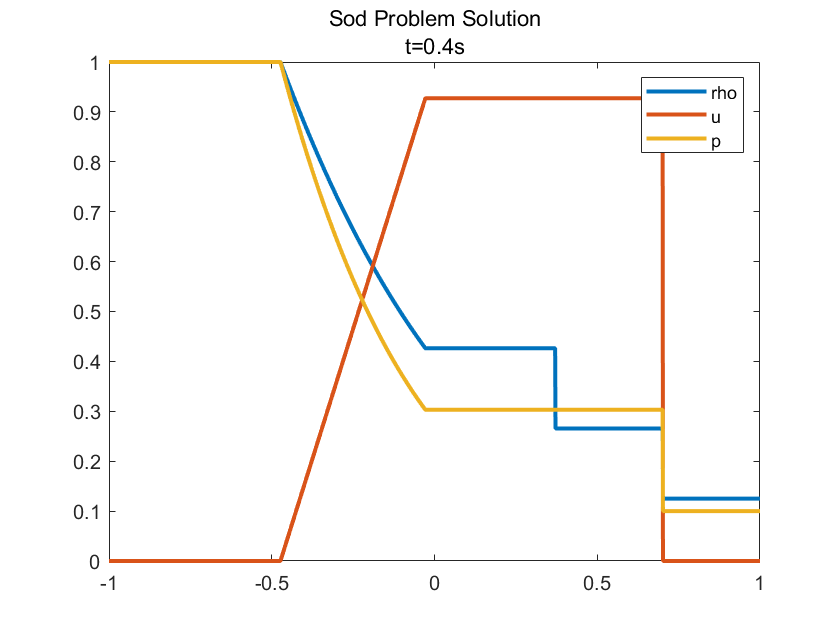
\includegraphics[width=\textwidth]{./fig/Riemann.png}
			\caption{\fontsize{10pt}{15pt}\selectfont Riemann精确解}
		\end{minipage}
		\end{figure}
		在结果图中我们可以看到,蓝线为密度$\rho$,红线为速度$u$,黄线为压强$p$,时间取最终时刻$t=0.4$。在生成的视频中我们可以看到,激波被由右区向右传播,接触间断处的密度发生突变而速度、压强平稳,膨胀波在左区向左传播,速度和密度呈平滑衰减过渡,这三个特征波组成了黎曼问题的解析解。
		
		通过构造中间状态($p^*,u^*$)并结合Rankine\_Hugoniot跃迁关系与膨胀自相似解,解析得到任意时刻下t的密度、速度与压强分布,反映了一维Euler系统中典型非线性波动的演化规律。
		
		\subsection{计算域网格大小的关系}
		以近似解中效果最好的NND+FVS+RK3求解方法为例,我们在LawOfDX.m文件中探究计算域网格大小对近似解求解效果的影响。
		
		我们分别设置$x \in [-1,1]$,设置空间间隔$dx=[0.1,0.05,0.01,0.005]$,设置$dt=0.001,t_{max} = 0.4$,依托NND+FVS+RK3的求解方法,得到不同空间间隔下关于速度$u$、压强$p$和密度$\rho$的数值解,将其与精确解画在一张图上,如图所示,可清晰观察到以下规律。
		\begin{enumerate}
			\item 整体趋势收敛明确。随着$dx$的减小,数值解逐渐向解析解收敛,误差明显减小,高分辨率(如$\Delta x = 0.005$下,数值解在各个间断与过渡区域都能精确捕捉波结构。
			\item 在激波与接触间断区域,误差随网格明显变化。对于$u$和$\rho$曲线,在$\Delta x = 0.1,0.05$时,激波后方和接触面区域出现数值扩散,表现为过渡层变宽、台阶不平;而在更精确的网格密度时,这些结构更陡峭,跳跃位置也更准确。
			\item 
			膨胀波区表现稳定但解析精度随网格提升而增强。$p$与$\rho$在膨胀波区域的变化较为平滑,表现出 WENO 格式在光滑区域的高阶精度;网格粗时略有数值耗散,网格细化后解变得更贴近解析光滑曲线。
			\item 数值解无明显振荡,方法稳定性良好。
		\end{enumerate}
		\begin{figure}[H]
		\centering
		\begin{minipage}{1\textwidth}
			\centering
			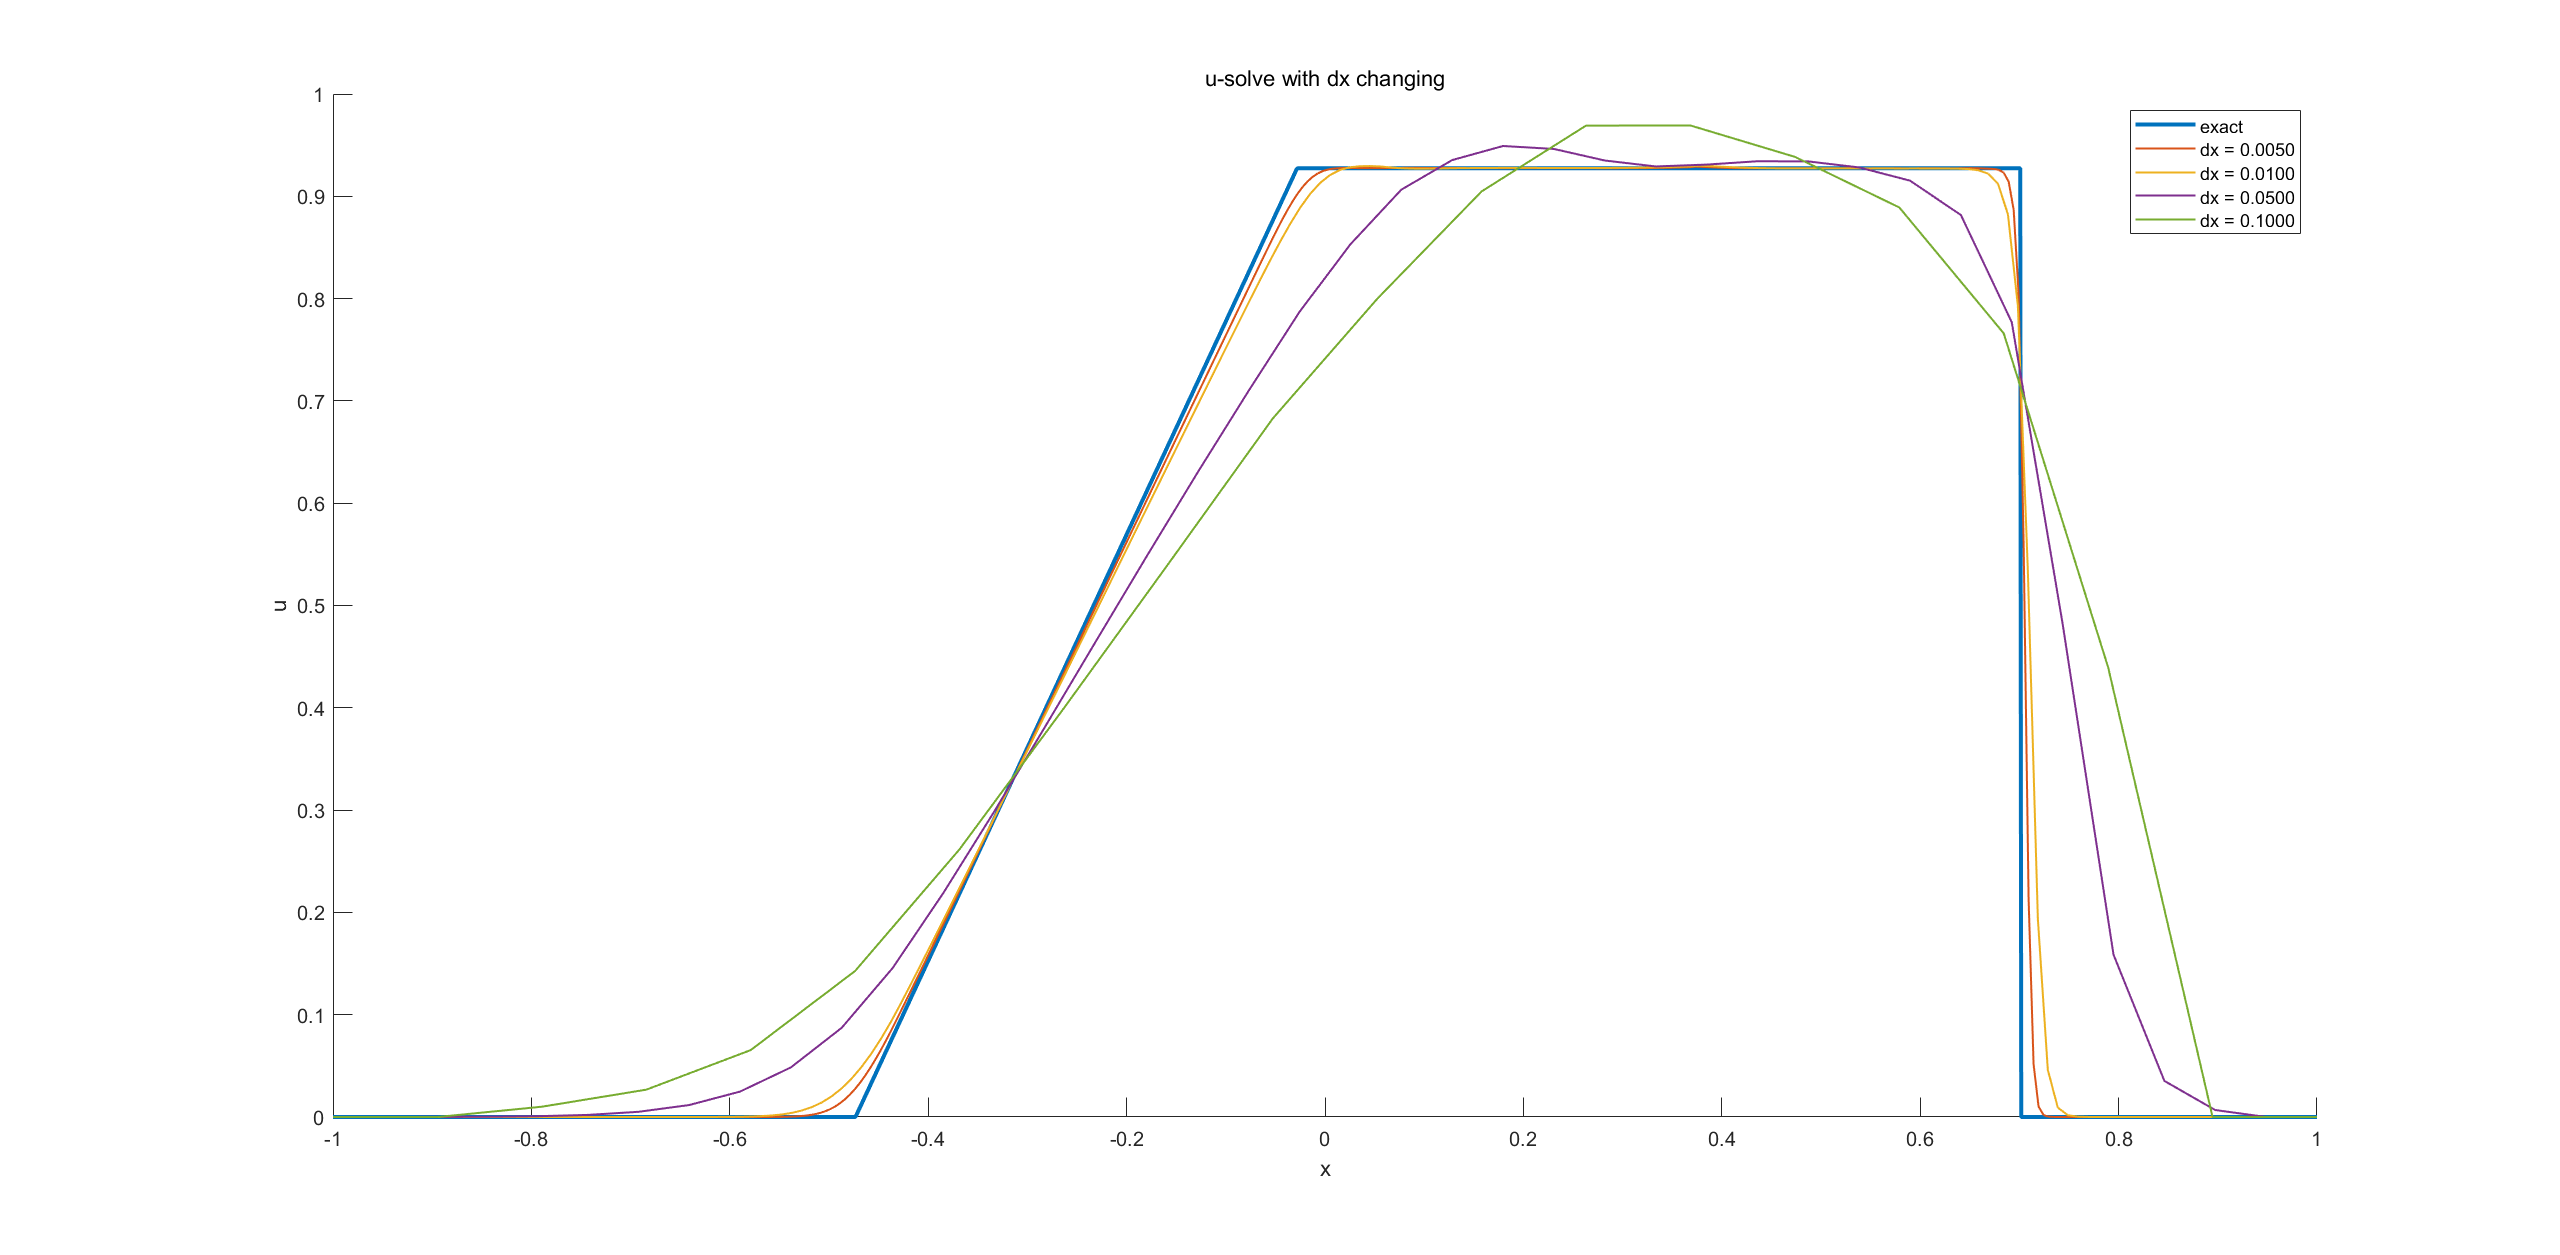
\includegraphics[width=\textwidth]{./fig/u.png}
			\caption{\fontsize{10pt}{15pt}\selectfont 不同网格精度下速度$u$的解曲线}
		\end{minipage}
		\end{figure}
		\begin{figure}[H]
			\centering
			\begin{minipage}{1\textwidth}
				\centering
				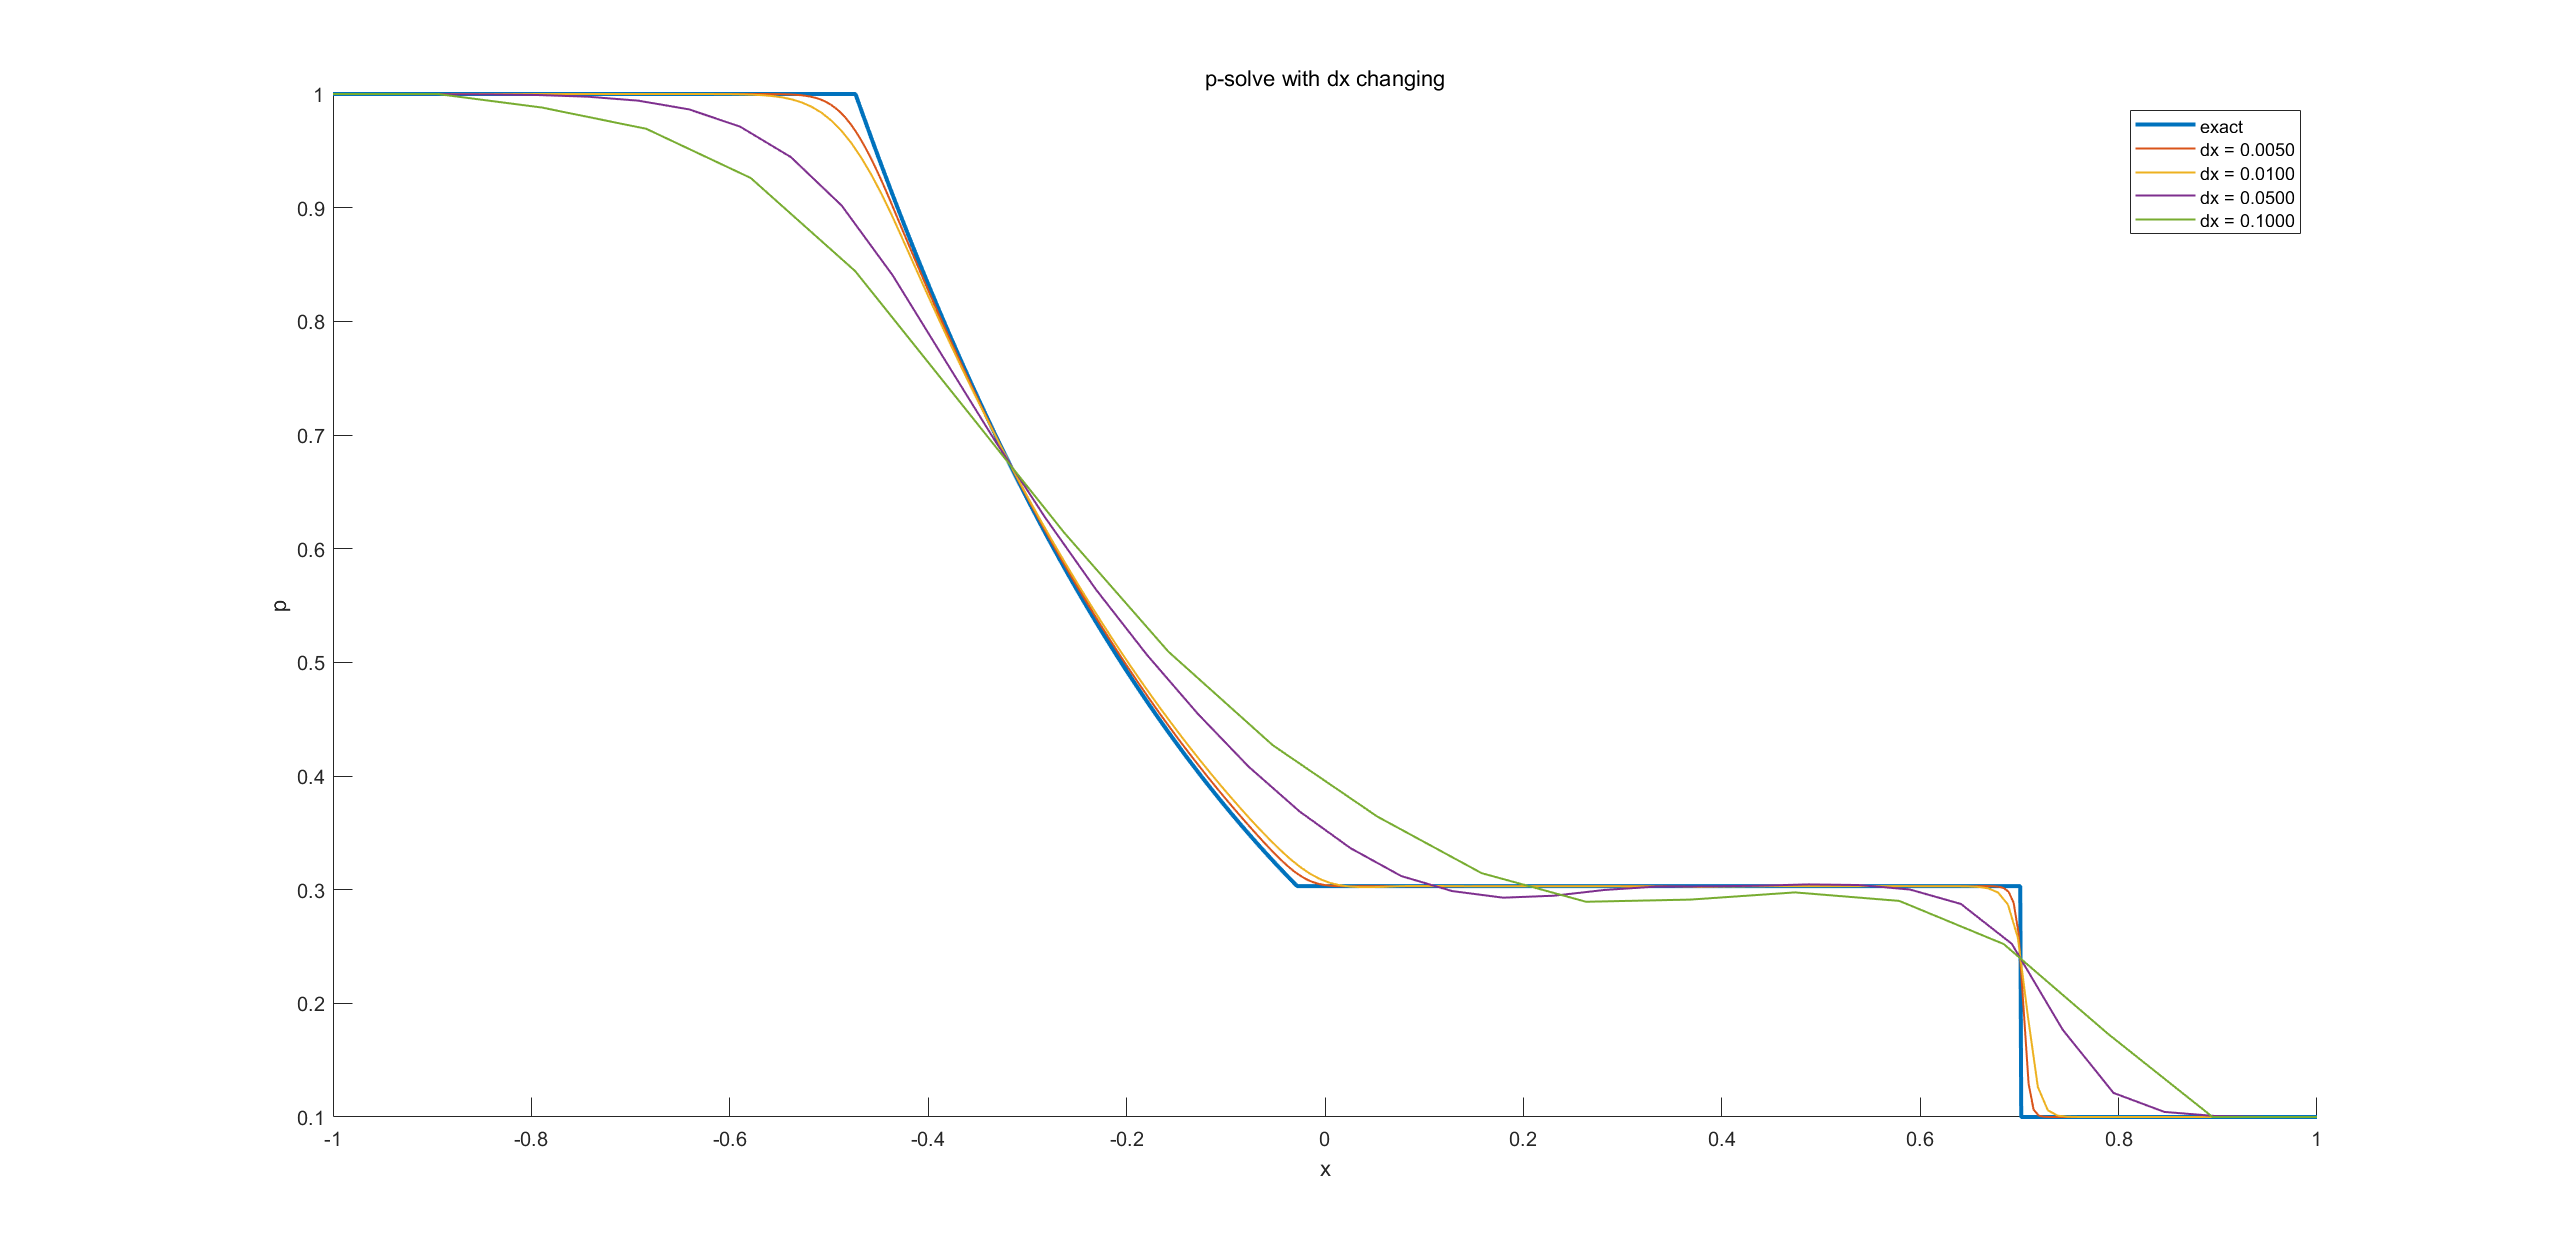
\includegraphics[width=\textwidth]{./fig/p.png}
				\caption{\fontsize{10pt}{15pt}\selectfont 不同网格精度下压强$p$的解曲线}
			\end{minipage}
		\end{figure}
		\begin{figure}[H]
			\centering
			\begin{minipage}{1\textwidth}
				\centering
				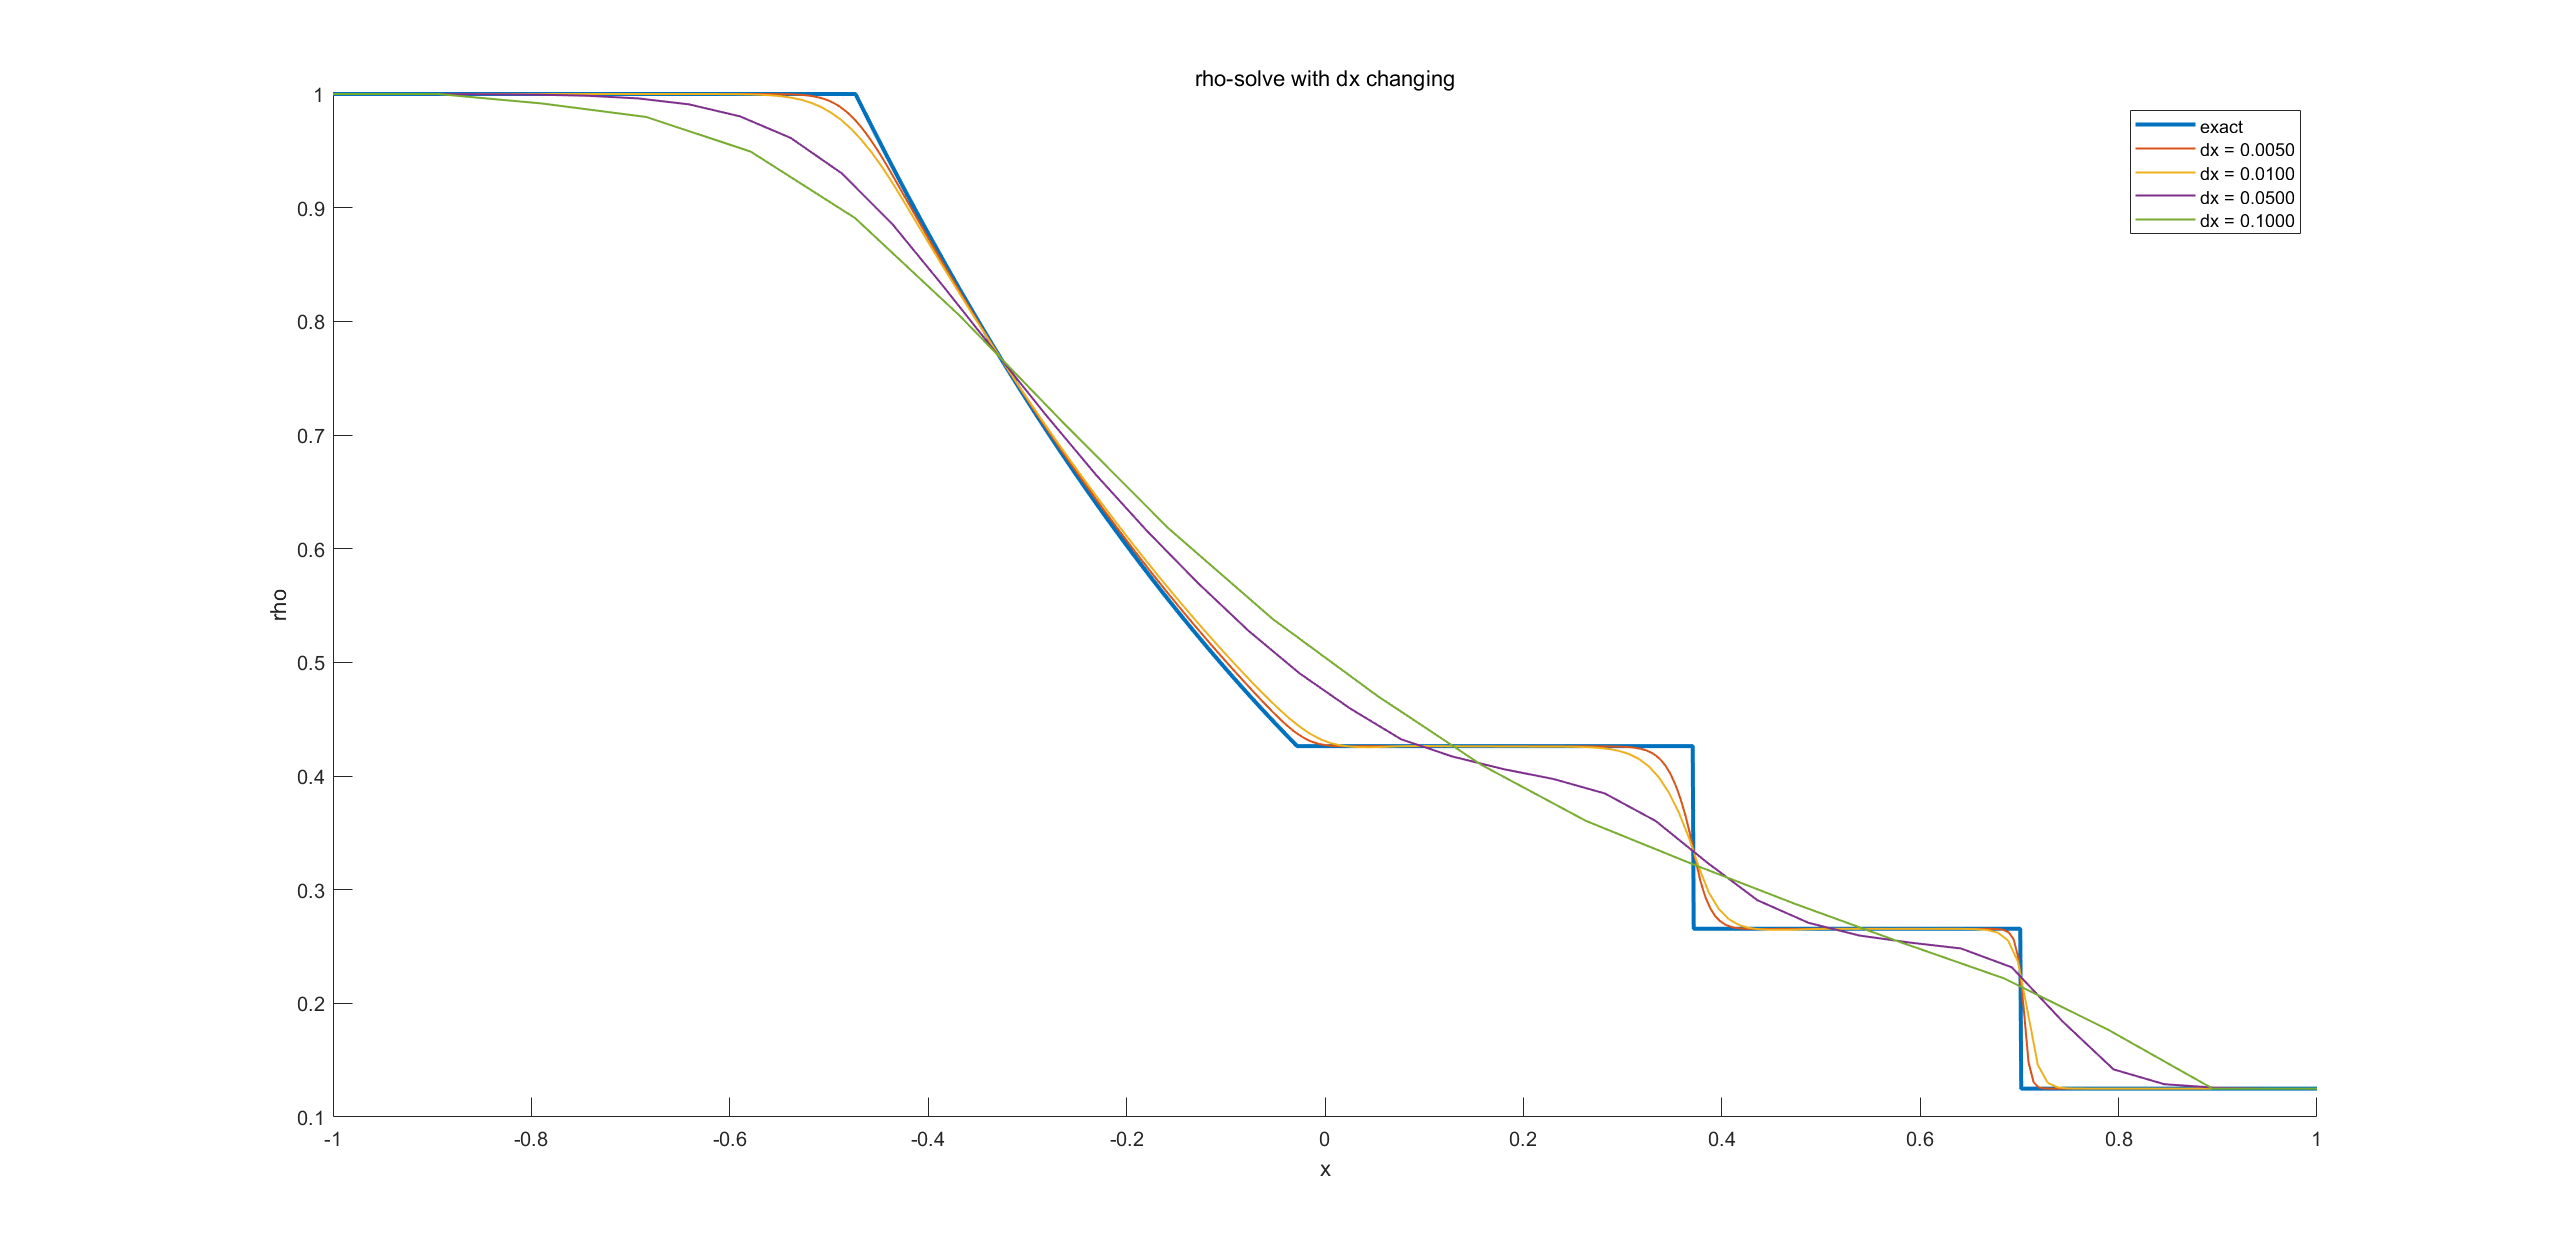
\includegraphics[width=\textwidth]{./fig/rho.png}
				\caption{\fontsize{10pt}{15pt}\selectfont 不同网格精度下密度$\rho$的解曲线}
			\end{minipage}
		\end{figure}
		整体而言,随着网格加密,数值解逐步逼近解析解,尤其在激波与接触面等间断区域表现出更高的分辨率和精度。
		
		
		\subsection{GVC+FVS+RK3方法}
		\begin{figure}[H]
			\centering
			\begin{minipage}{1\textwidth}
				\centering
				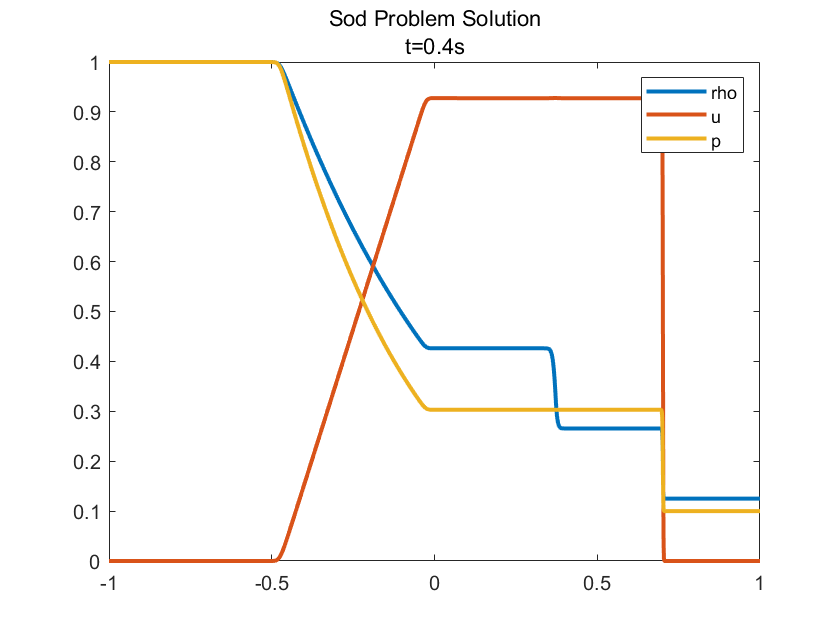
\includegraphics[width=\textwidth]{./fig/app1.png}
				\caption{\fontsize{10pt}{15pt}\selectfont GVC+FVS+RK3方法近似解}
			\end{minipage}
		\end{figure}
		NND格式实现空间高阶重构,FVS方法处理通量,三阶RungeKutta格式进行时间推进。该组合兼具震波捕捉能力与无振荡性。左侧膨胀波区域密度与压强呈连续下降,速度线性上升,曲线形状平滑,较好还原解析解中的稀疏波;中间密度出现轻微但清晰的阶跃,速度与压强保持连续,未出现明显数值振荡,具有良好的非振荡性;右侧激波区域阶跃较为准确,表现出激波捕捉方面的稳健性。
		
		\subsection{WENO+FDS+RK3方法}
		\begin{figure}[H]
			\centering
			\begin{minipage}{1\textwidth}
				\centering
				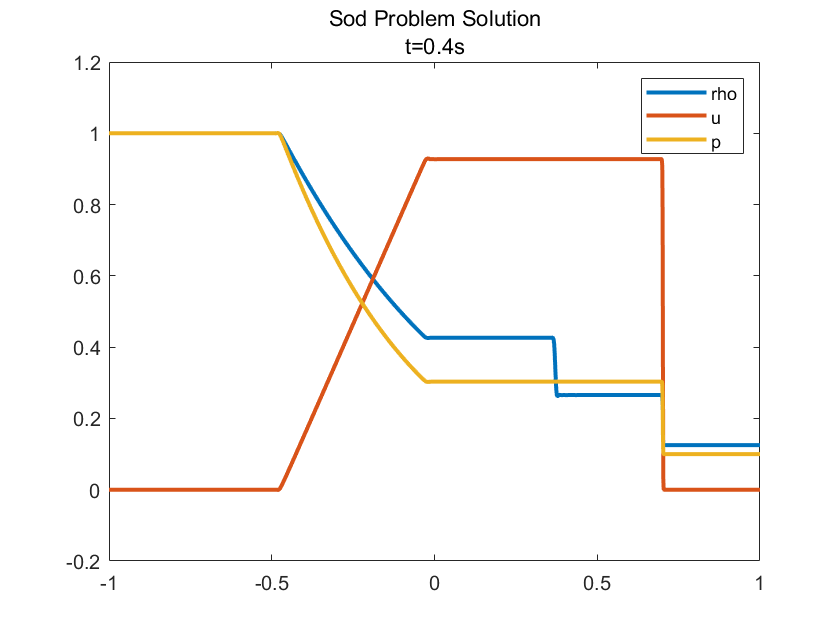
\includegraphics[width=\textwidth]{./fig/app2.png}
				\caption{\fontsize{10pt}{15pt}\selectfont WENO+FDS+RK3方法近似解}
			\end{minipage}
		\end{figure}
		五阶WENO重构提升间断捕捉精度,基于波速分裂的HLLC的计算通量公式,显式三阶Runge-Kutta方法保持整体三阶时间精度构成了求近似解的组合。左侧膨胀波区域密度和压强平滑下降,速度线性上升,由于WENO方法在光滑区展现的高阶精度,几乎无数值耗散;中间接触间断处密度存在阶跃,压强和速度保持连续,接触面过渡范围小说明该组合高分辨率,且无明显数值振荡;右侧激波清晰紧凑,表明对激波结构捕捉良好的保形性。
		
		
		\subsection{TVD方法}
		\begin{figure}[H]
			\centering
			\begin{minipage}{1\textwidth}
				\centering
				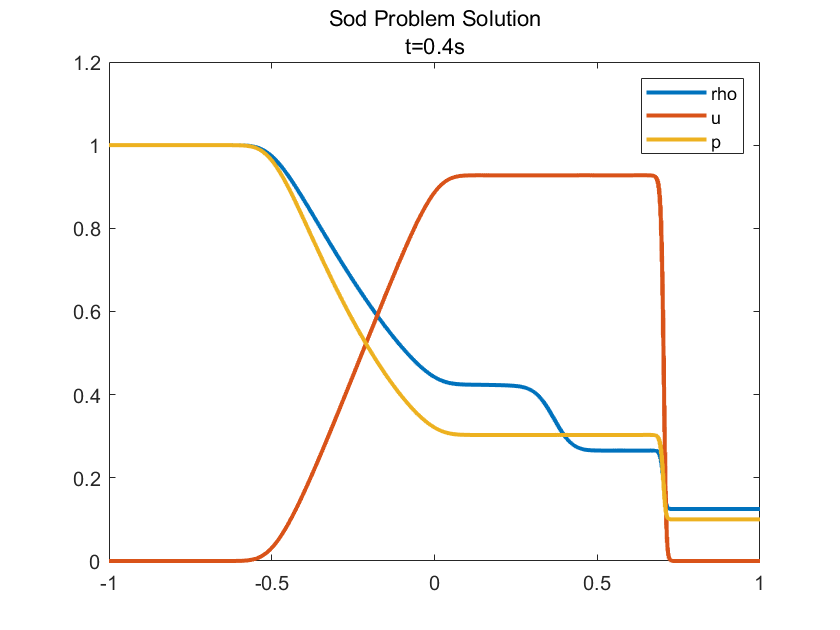
\includegraphics[width=\textwidth]{./fig/app3.png}
				\caption{\fontsize{10pt}{15pt}\selectfont TVD方法近似解}
			\end{minipage}
		\end{figure}
		TVD实现激波捕捉,确保总变差不增加,具有良好的稳定性和抑制非物理振荡的能力。从图中我们可以观察到,左侧膨胀波区域密度与压强光滑下降,速度连续上升,曲线过渡平稳,未见数值振荡,说明TVD格式成功保留了解的光滑性;中间接触间断处密度出现明显突变,速度与压强保持连续,阶跃未出现伪影,表明限制器有效限制了局部振荡;右侧激波区域密度、压强和速度出现阶跃,虽有一定程度的扩散,但位置准确,无数值震荡。
			
		\subsection{总结}
		我们将三种方法结果与精确解置于一张图,并总结如下表:
		\begin{figure}[H]
			\centering
			\begin{minipage}{1\textwidth}
				\centering
				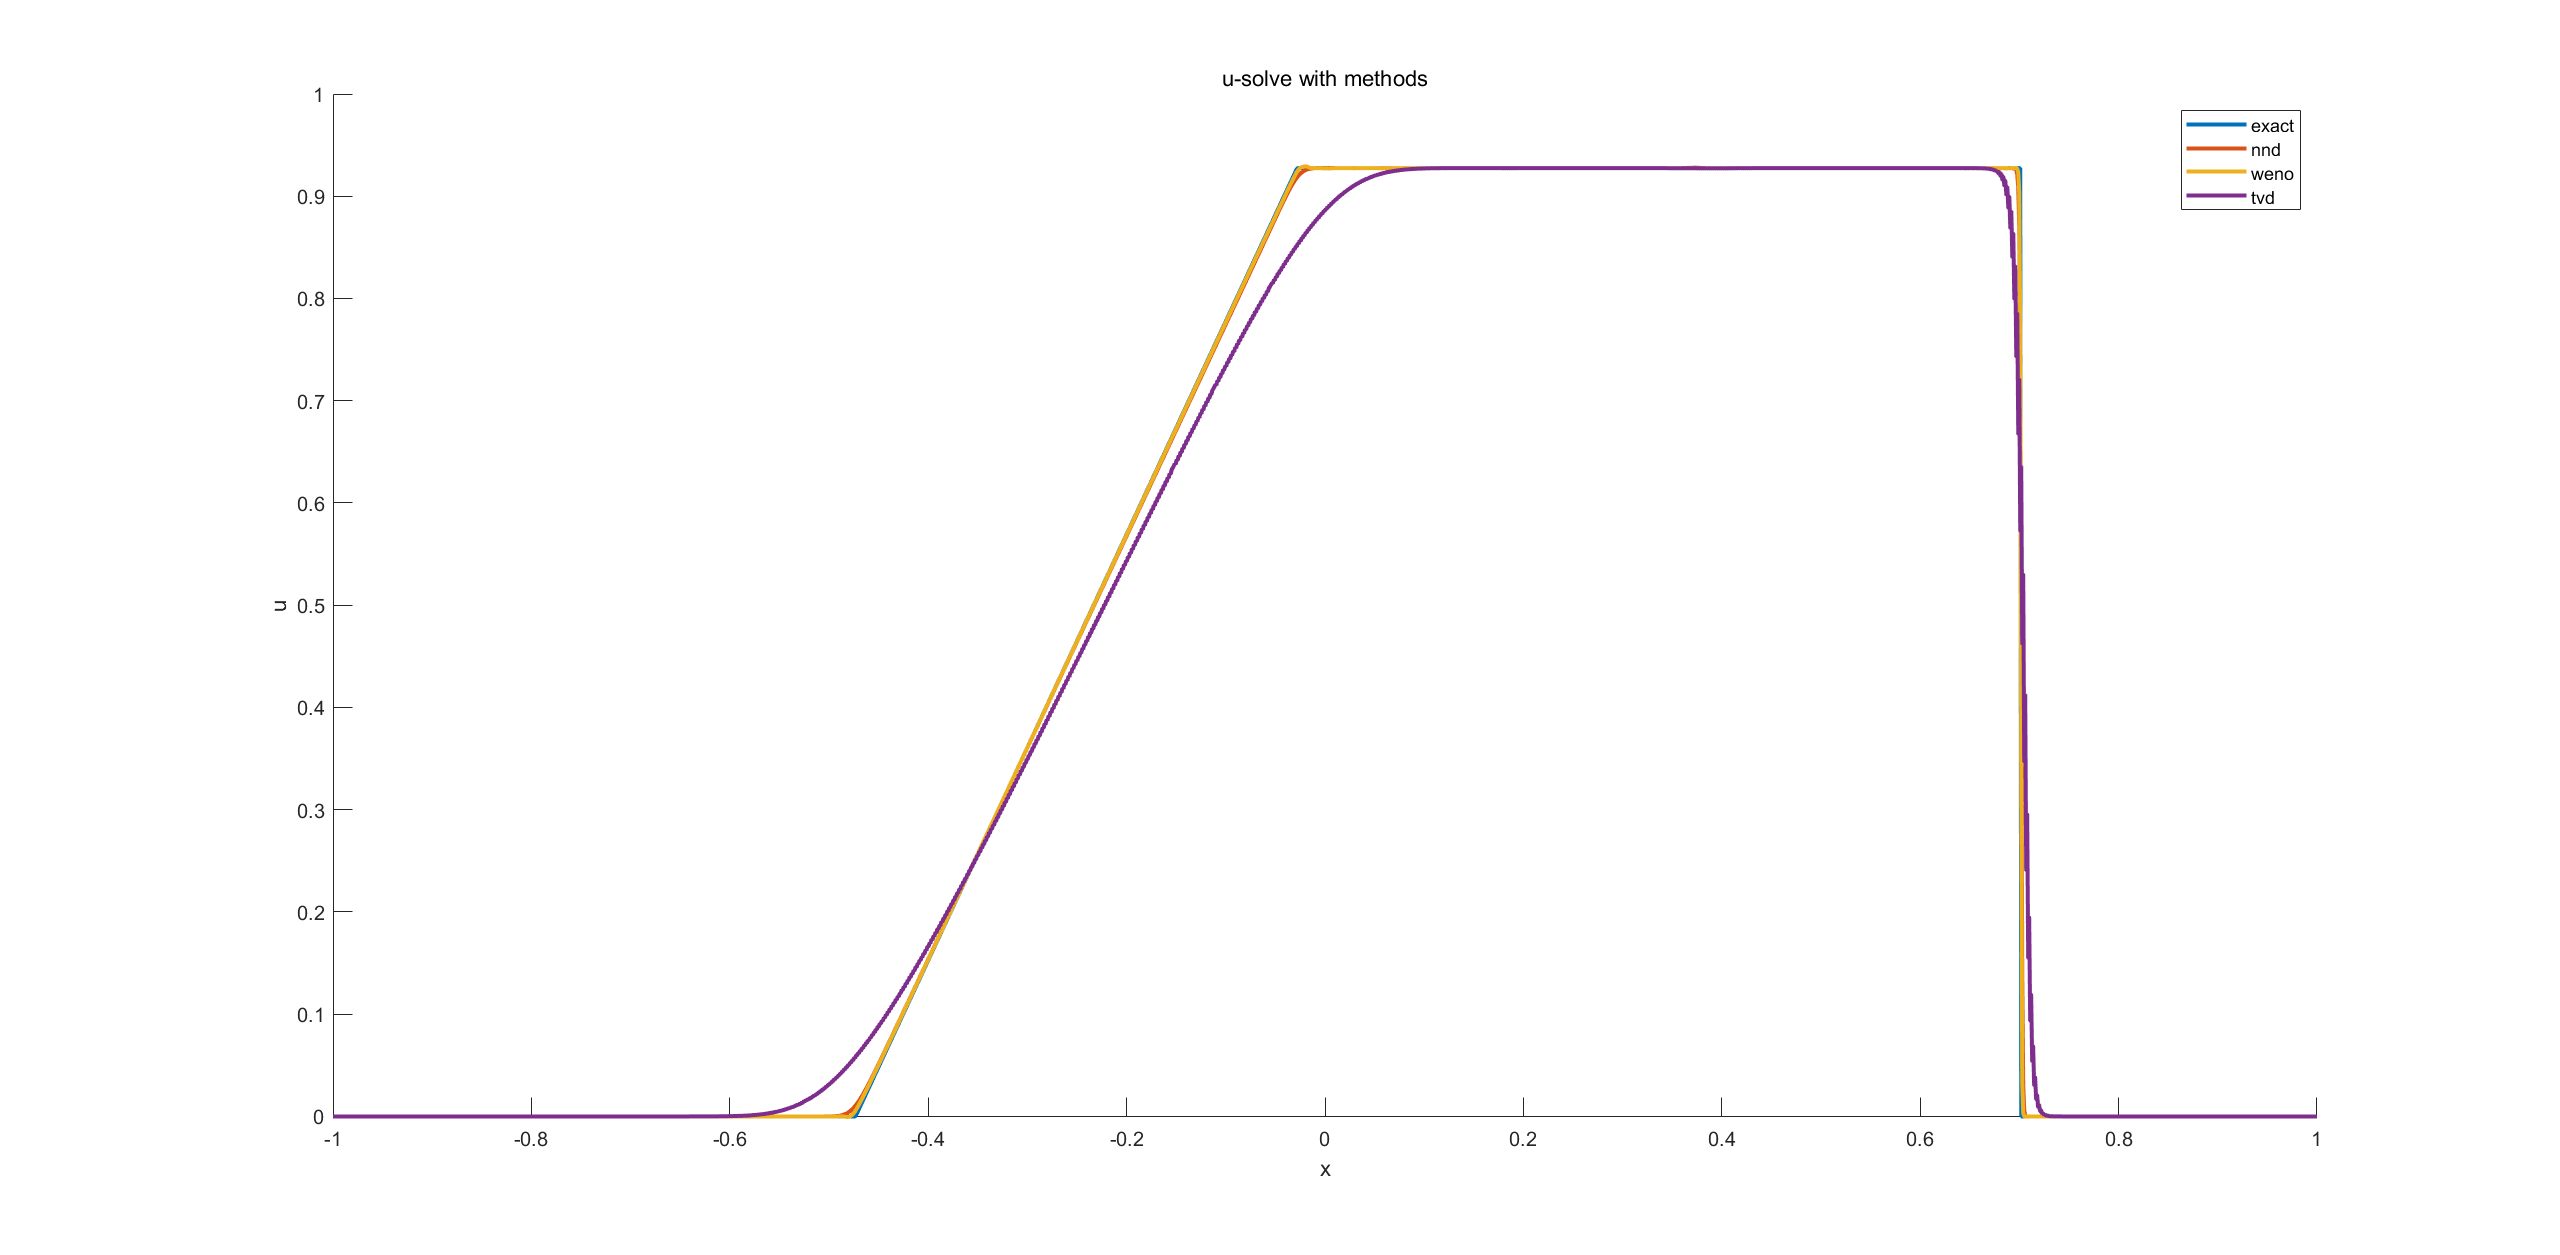
\includegraphics[width=\textwidth]{./fig/u-2.png}
				\caption{\fontsize{10pt}{15pt}\selectfont 不同求解方法速度$u$的解曲线}
			\end{minipage}
		\end{figure}
		\begin{figure}[H]
			\centering
			\begin{minipage}{1\textwidth}
				\centering
				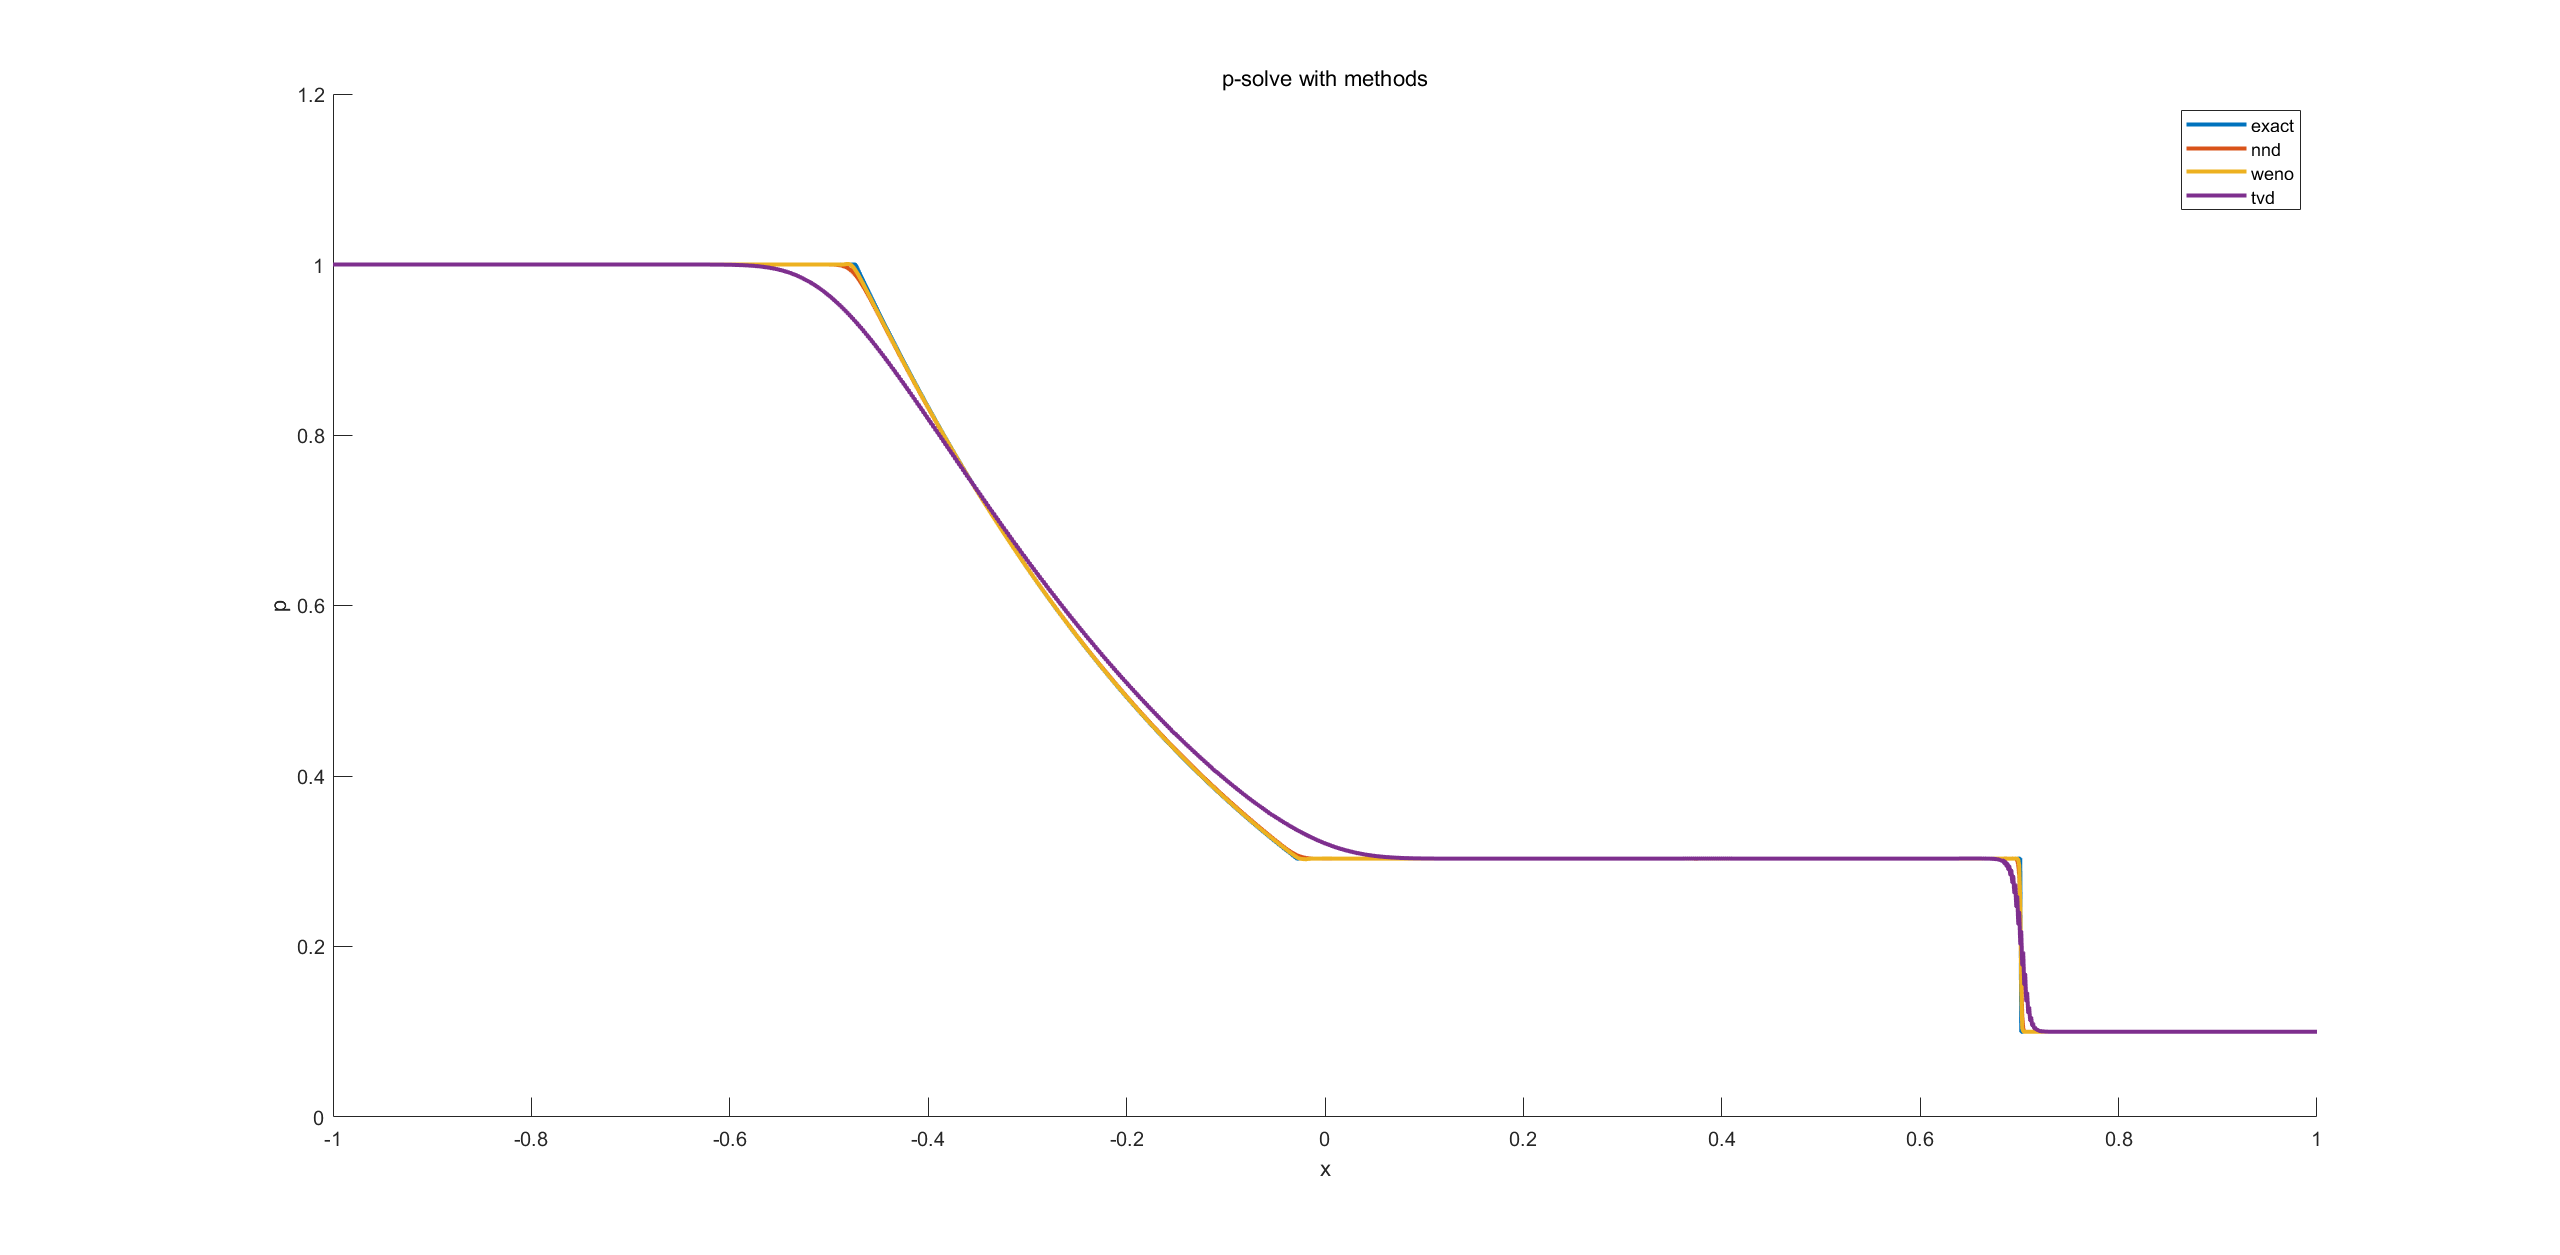
\includegraphics[width=\textwidth]{./fig/p-2.png}
				\caption{\fontsize{10pt}{15pt}\selectfont 不同求解方法压强$p$的解曲线}
			\end{minipage}
		\end{figure}
		\begin{figure}[H]
			\centering
			\begin{minipage}{1\textwidth}
				\centering
				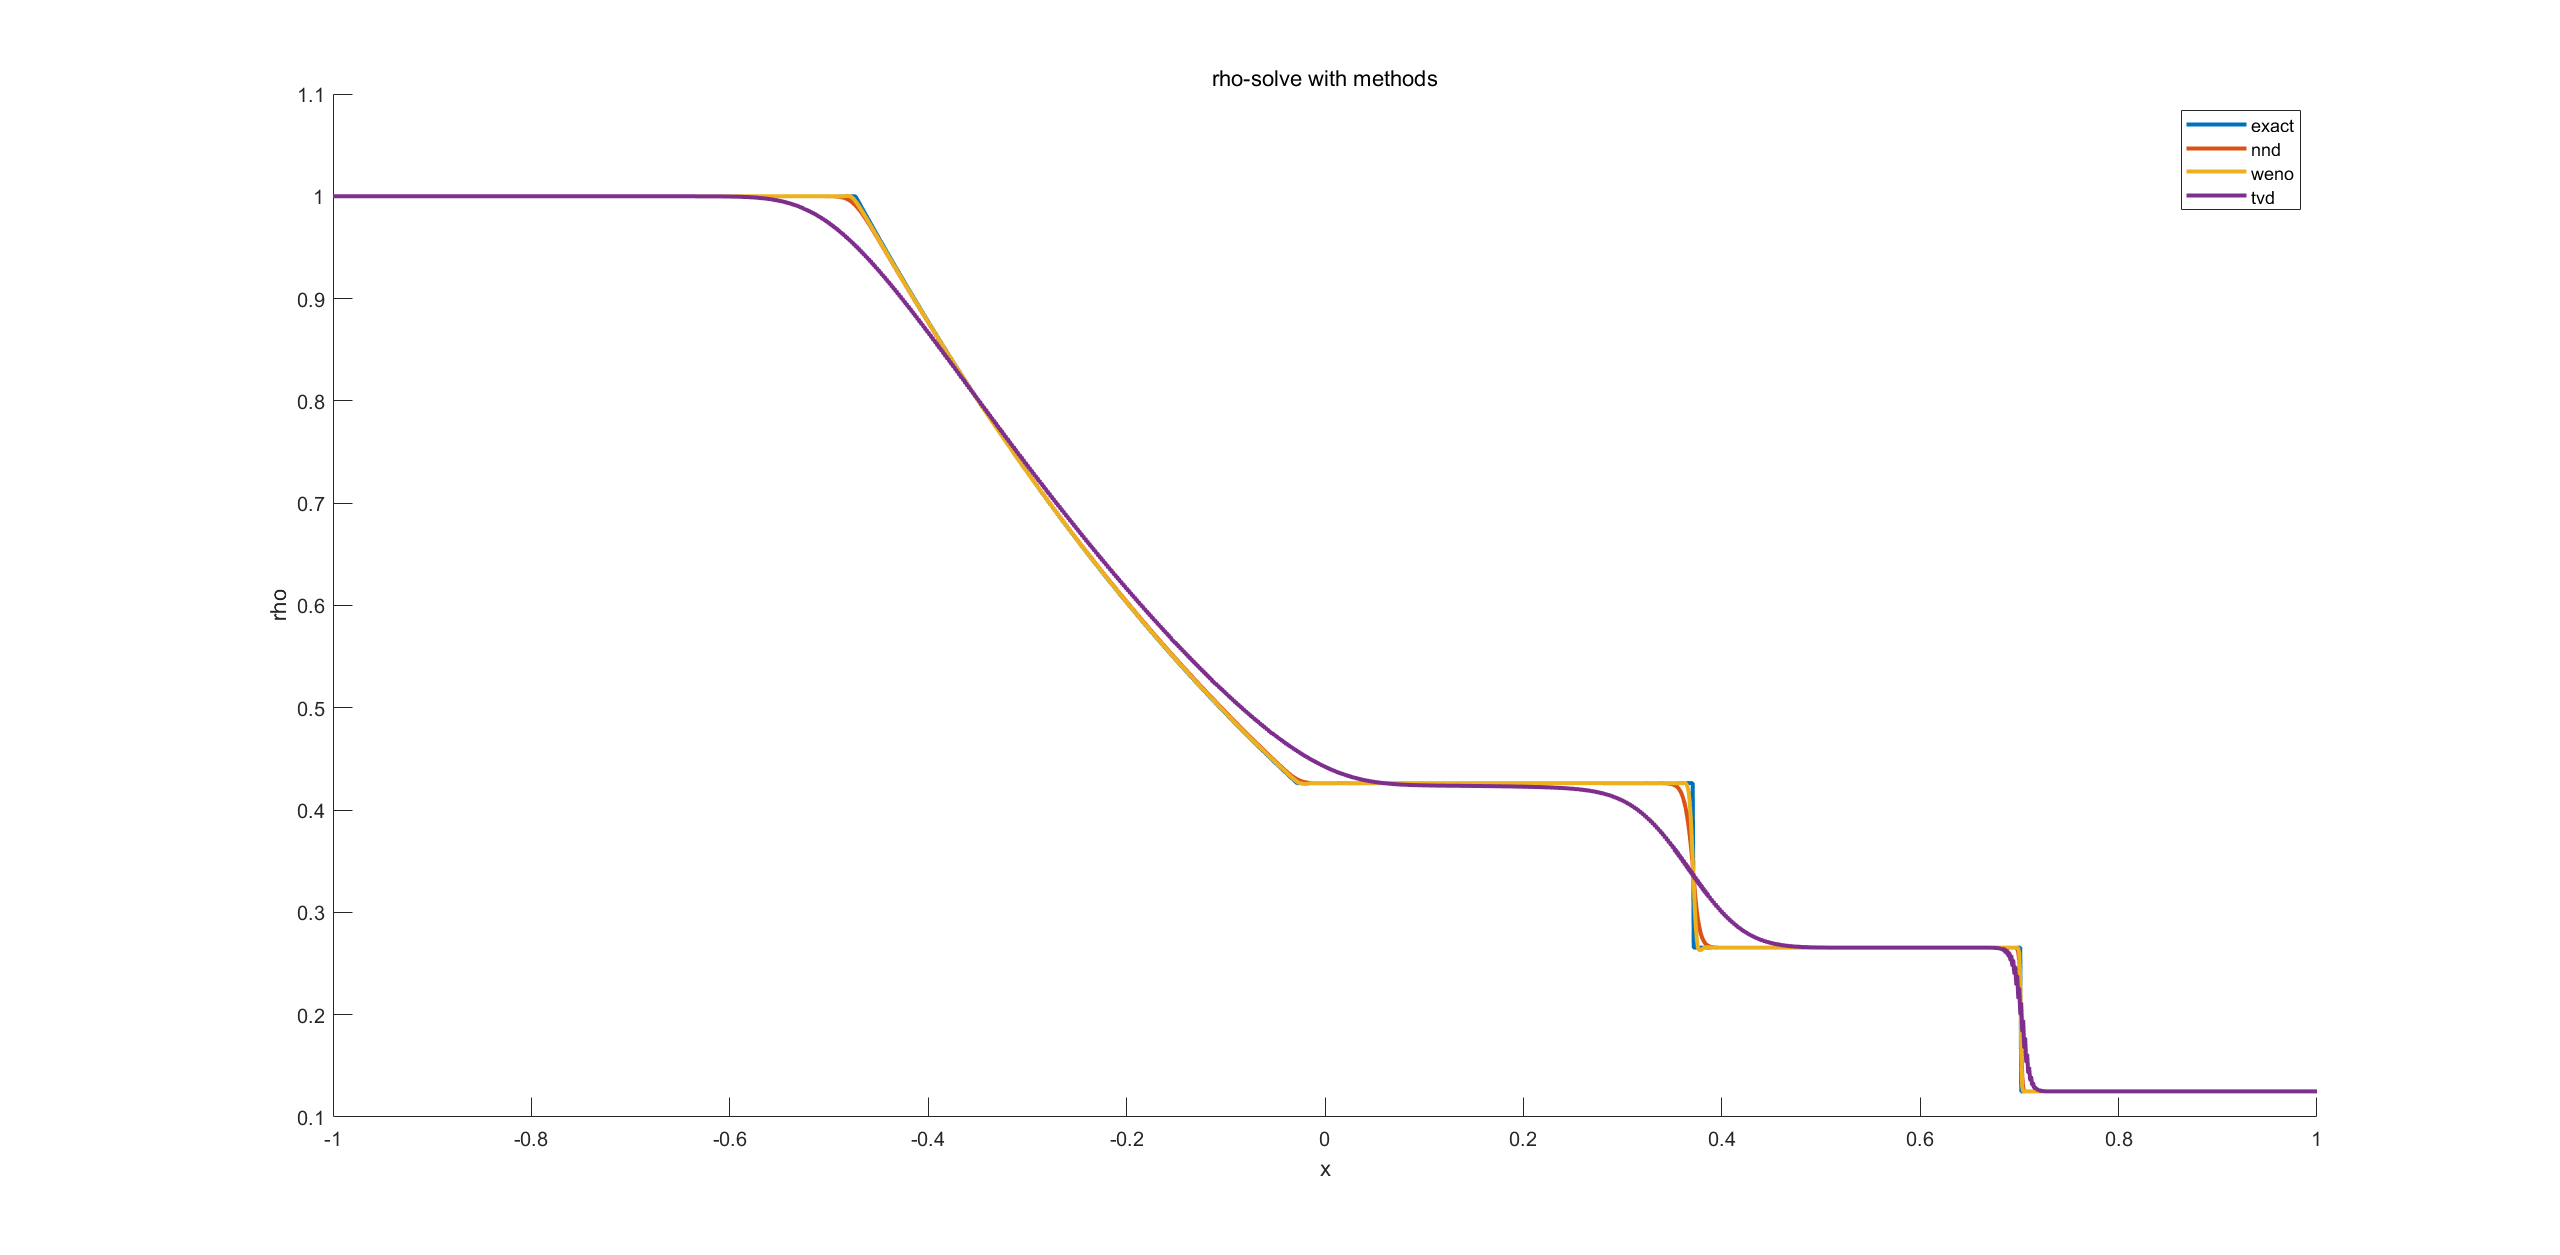
\includegraphics[width=\textwidth]{./fig/rho-2.png}
				\caption{\fontsize{10pt}{15pt}\selectfont 不同求解方法密度$\rho$的解曲线}
			\end{minipage}
		\end{figure}
		图中将数值解与精确解进行对比,分别在三个物理量上呈现,不难看出各格式都能基本还原解的整体结构:膨胀波、接触间断和激波均可辨认;但在接触间断精度、激波过渡宽度、波前稳定性方面存在显著差异。
		
		TVD方法表现为最稳定的格式,几乎无数值振荡;但数值耗散最强,导致激波和接触面附近的跳跃区域变宽、变平缓;精度较低,但具有优秀的鲁棒性,适合粗网格/强间断问题。
		
		WENO+FDS方法在所有方法中表现出最好的高阶精度,膨胀波区平滑;激波位置贴合精确解;接触面跳跃更集中;略有小幅“台阶状”误差,原因可能是未使用特征重构或误差扩展到能量项;在分辨率和精度上达到较好平衡。
		
		NND+FVS方法表现介于TVD和WENO之间,相较于 TVD 有更清晰的跳跃结构;相较于 WENO,仍略显扩散,特别是在接触面区域;稳定性优于 WENO,误差略大于其,但收敛速度较好。
		
		\begin{table}[H]
			\centering
			\caption{三种格式的比较结果}
			\begin{tabular}{lccc}
				\toprule
				特征维度 & TVD & WENO+FDS & NND+FVS \\
				\midrule
				振荡性       & 轻微振荡,较稳定   & 无振荡,较稳定     & 基本无振荡 \\
				分辨率  & 接触面略有数值扩散     & 高分辨率,锐利分界   & 平衡稳定性与分辨率 \\
				算法复杂度   & 简单,易于实现   & 复杂,需进行权重处理     & 略复杂,依赖重构方式 \\
				计算效率 & 快速稳定 & 耗时多,重构成本较高 & 中等 \\
				物理一致性 & 间断处有钝化趋势 & 精度高重 & 稳定守恒,非振荡性好 \\
				\bottomrule
			\end{tabular}
		\end{table}
		
	\section{附加题}
	\subsection{数学原理}
		为了将特征重构法应用与FVS框架,我们采用基于NND+FVS+RK3.m代码文件,将NND格式改为特征重构保存与REC+FVS+RK3.m代码文件中。
		
		特征重构的不同点在于,将非线性项$\frac{\partial F}{\partial x}$改为$A\frac{\partial U}{\partial x}$,从而对$A$进行特征变换,在特征空间中计算通量$F$。
		
		考虑方程组
		\[
		\frac{\partial U}{\partial t} + \frac{\partial F}{\partial x} = 0 
		\]
		非守恒形式为
		\[
		\frac{\partial U}{\partial t} + A \frac{\partial U}{\partial x} = 0
		\]
		其中 $A = \frac{\partial F}{\partial U}$。这里 $U$ 和 $F$ 都是 $n$ 维矢量函数,$A$ 是 $n \times n$ 矩阵。由于方程组是双曲型的,要求矩阵 $A$ 有 $n$ 个实特征值,于是存在右特征向量矩阵 $R$,使得
		\[
		A = R \Lambda R^{-1}
		\]
		这里 $\Lambda = \mathrm{diag}(\lambda_1, \lambda_2, \cdots, \lambda_n)$ 为对角矩阵,$\lambda_i$ 是矩阵 $A$ 的特征值。引入向量 $W = R^{-1} U$,并以矩阵 $R^{-1}$ 左乘(7.114),得到
		\[
		\frac{\partial W}{\partial t} + \Lambda \frac{\partial W}{\partial x} = 0
		\]
		由于 $\Lambda$ 是对角矩阵,上方程组可写为分量形式:
		\[
		\frac{\partial w_i}{\partial t} + \lambda_i \frac{\partial w_i}{\partial x} = 0, \quad (i = 1, 2, \ldots, n)
		\]
		这已经是一个标量方程,对于它可以使用前面的 NND 格式,也就是说对方程(7.116)可以直接写出其 NND 格式。在将格式的表达式再回到左乘矩阵 $R$,便得到关于方程(7.113)的 NND 格式。为了表示的方便,引入对角矩阵的分解:
		\[
		\Lambda = \Lambda^+ + \Lambda^- = \mathrm{diag}(\lambda_1^+, \ldots, \lambda_n^+) + \mathrm{diag}(\lambda_1^-, \ldots, \lambda_n^-)
		\]
		其中,
		\[
		\lambda_i^{\pm} = \frac{\lambda_i \pm |\lambda_i|}{2}, \quad (i = 1, 2, \ldots, n)
		\]
		进一步可以引入矩阵 $A$ 的分解:
		\[
		A = A^+ + A^- = R \Lambda^+ R^{-1} + R \Lambda^- R^{-1}
		\]
		于是可得到关于通量 $\mathbf{F}$ 的分解:
		\[
		F = F^+ + F^- = A^+ U + A^- U
		\]
		这样再利用FVS通量分解法进行通量计算,即成功将特征重构应用于FVS框架中。
		
		\subsection{代码编写}
		我们在REC\_FVS\_RK3.m文件中完成对Sod问题的近似求解。算法流程大致分为以下几个步骤:
		\begin{enumerate}
			\item 计算声速和特征值。
			\item 根据特征重构法格式计算每个位置的通量及守恒量。
			\item 根据NND通量分解格式计算每个位置的守恒量
			\item 利用Runge-Kutta方法完成时间步推进。
			\item 将每次计算结果重画在画布上,方便展示结果动态变化过程,同时方便我们生成视频。
		\end{enumerate}
		
		\subsection{结果讨论}
		\begin{figure}[H]
			\centering
			\begin{minipage}{1\textwidth}
				\centering
				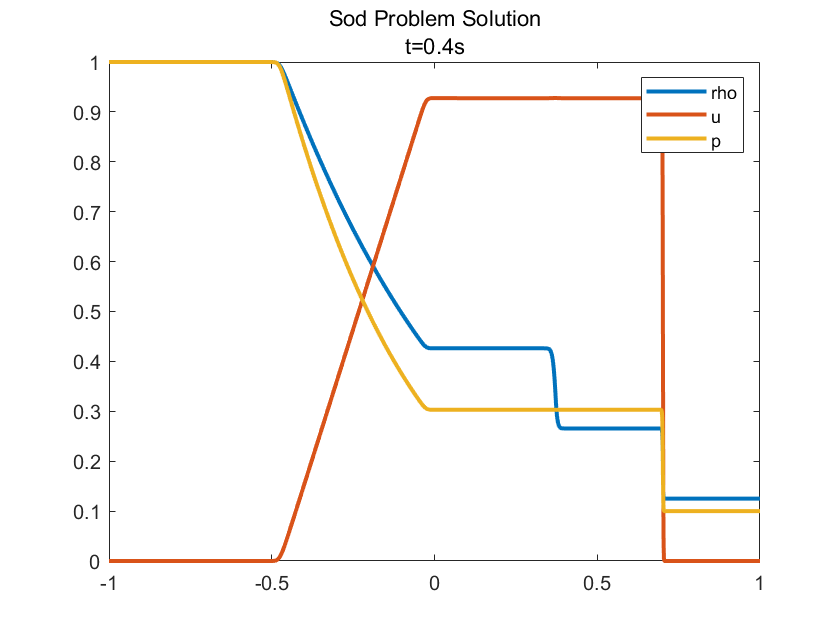
\includegraphics[width=\textwidth]{./fig/app4.png}
				\caption{\fontsize{10pt}{15pt}\selectfont 特征重构方法近似解}
			\end{minipage}
		\end{figure}
		\begin{figure}[H]
			\centering
			\begin{minipage}{1\textwidth}
				\centering
				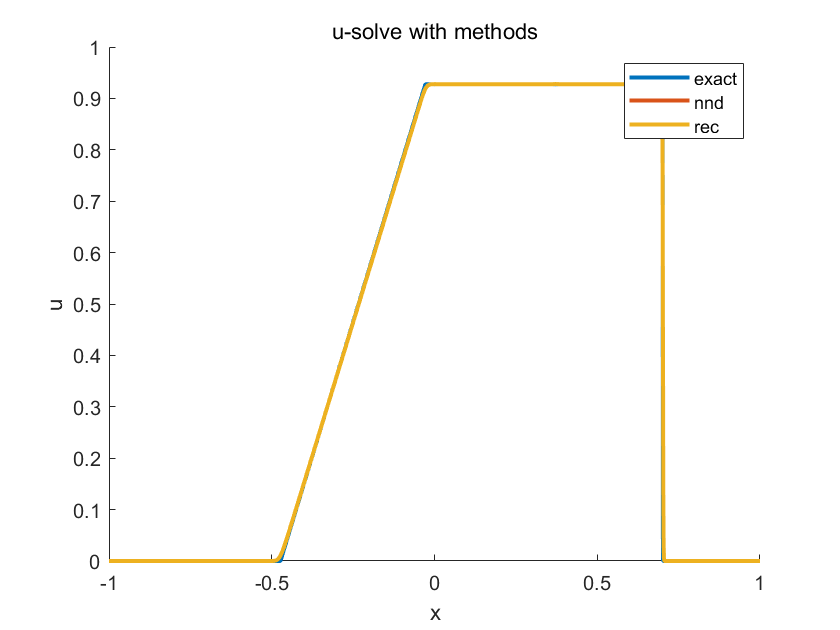
\includegraphics[width=\textwidth]{./fig/u-3.png}
				\caption{\fontsize{10pt}{15pt}\selectfont 特征重构方法于保守量方法对比(速度$u$)}
			\end{minipage}
		\end{figure}
		\begin{figure}[H]
			\centering
			\begin{minipage}{1\textwidth}
				\centering
				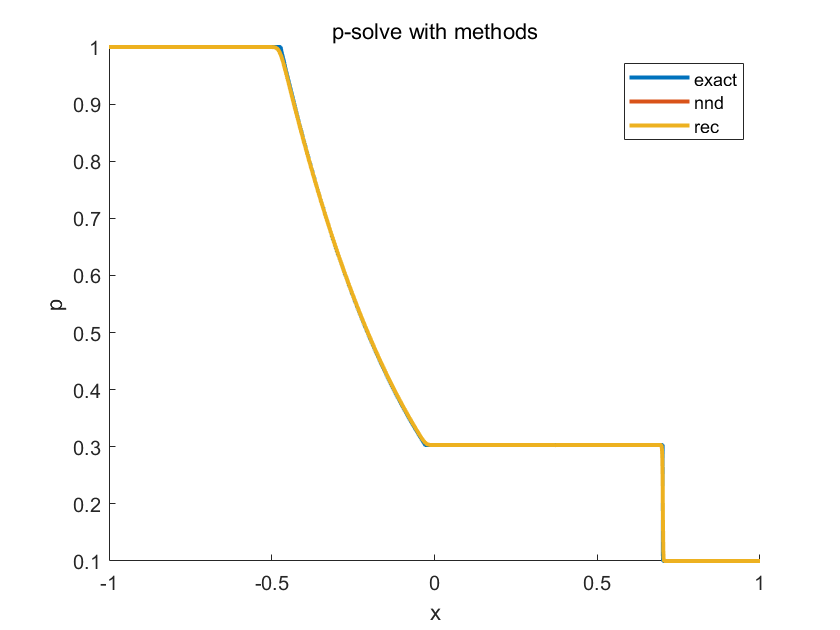
\includegraphics[width=\textwidth]{./fig/p-3.png}
				\caption{\fontsize{10pt}{15pt}\selectfont 特征重构方法于保守量方法对比(压强$p$)}
			\end{minipage}
		\end{figure}
		\begin{figure}[H]
			\centering
			\begin{minipage}{1\textwidth}
				\centering
				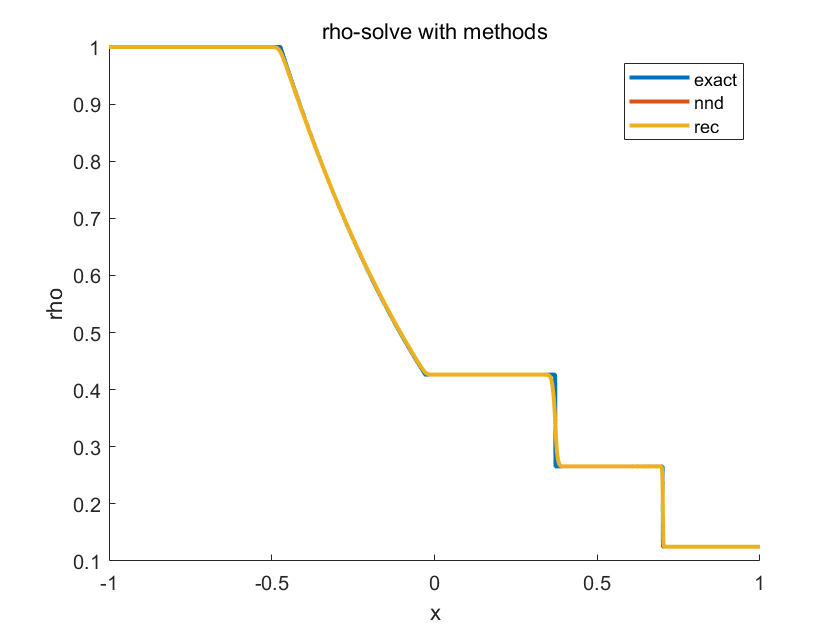
\includegraphics[width=\textwidth]{./fig/rho-3.png}
				\caption{\fontsize{10pt}{15pt}\selectfont 特征重构方法于保守量方法对比(密度$\rho$)}
			\end{minipage}
		\end{figure}
		图中显示了在特征变量空间中使用 NND 重构格式所得到的 Sod 激波问题数值解。整体解结构良好,各变量间断清晰、平滑区域高保真,未出现非物理震荡。图中保守变量与特征重构法的解相差不大是因为空间离散精度足够高。当空间离散精度降低时,与保守变量上的 NND 格式相比,特征重构显著提升了解的稳定性与局部保形性,尤其在接触间断与激波捕捉方面更为准确。结果表明,特征重构对于降低变量耦合带来的误差传播、提升非振荡性具有明显作用,是一种值得推广的改进策略。
		
		
	\section{附录}
		\begin{enumerate}
			\item Github管理说明:
			本项目存于RobertRainbow/CFDFinal/的仓库中,具体分为:README.md文件用于帮助用户了解仓库代码结构及内容;Request.pdf文件为大作业要求;Report文件夹为latex语言完成报告相关文件;Code文件夹为matlab代码用于求解本作业问题。管理记录见图:
			\begin{figure}[H]
				\centering
				\begin{minipage}{0.83\textwidth}
					\centering
					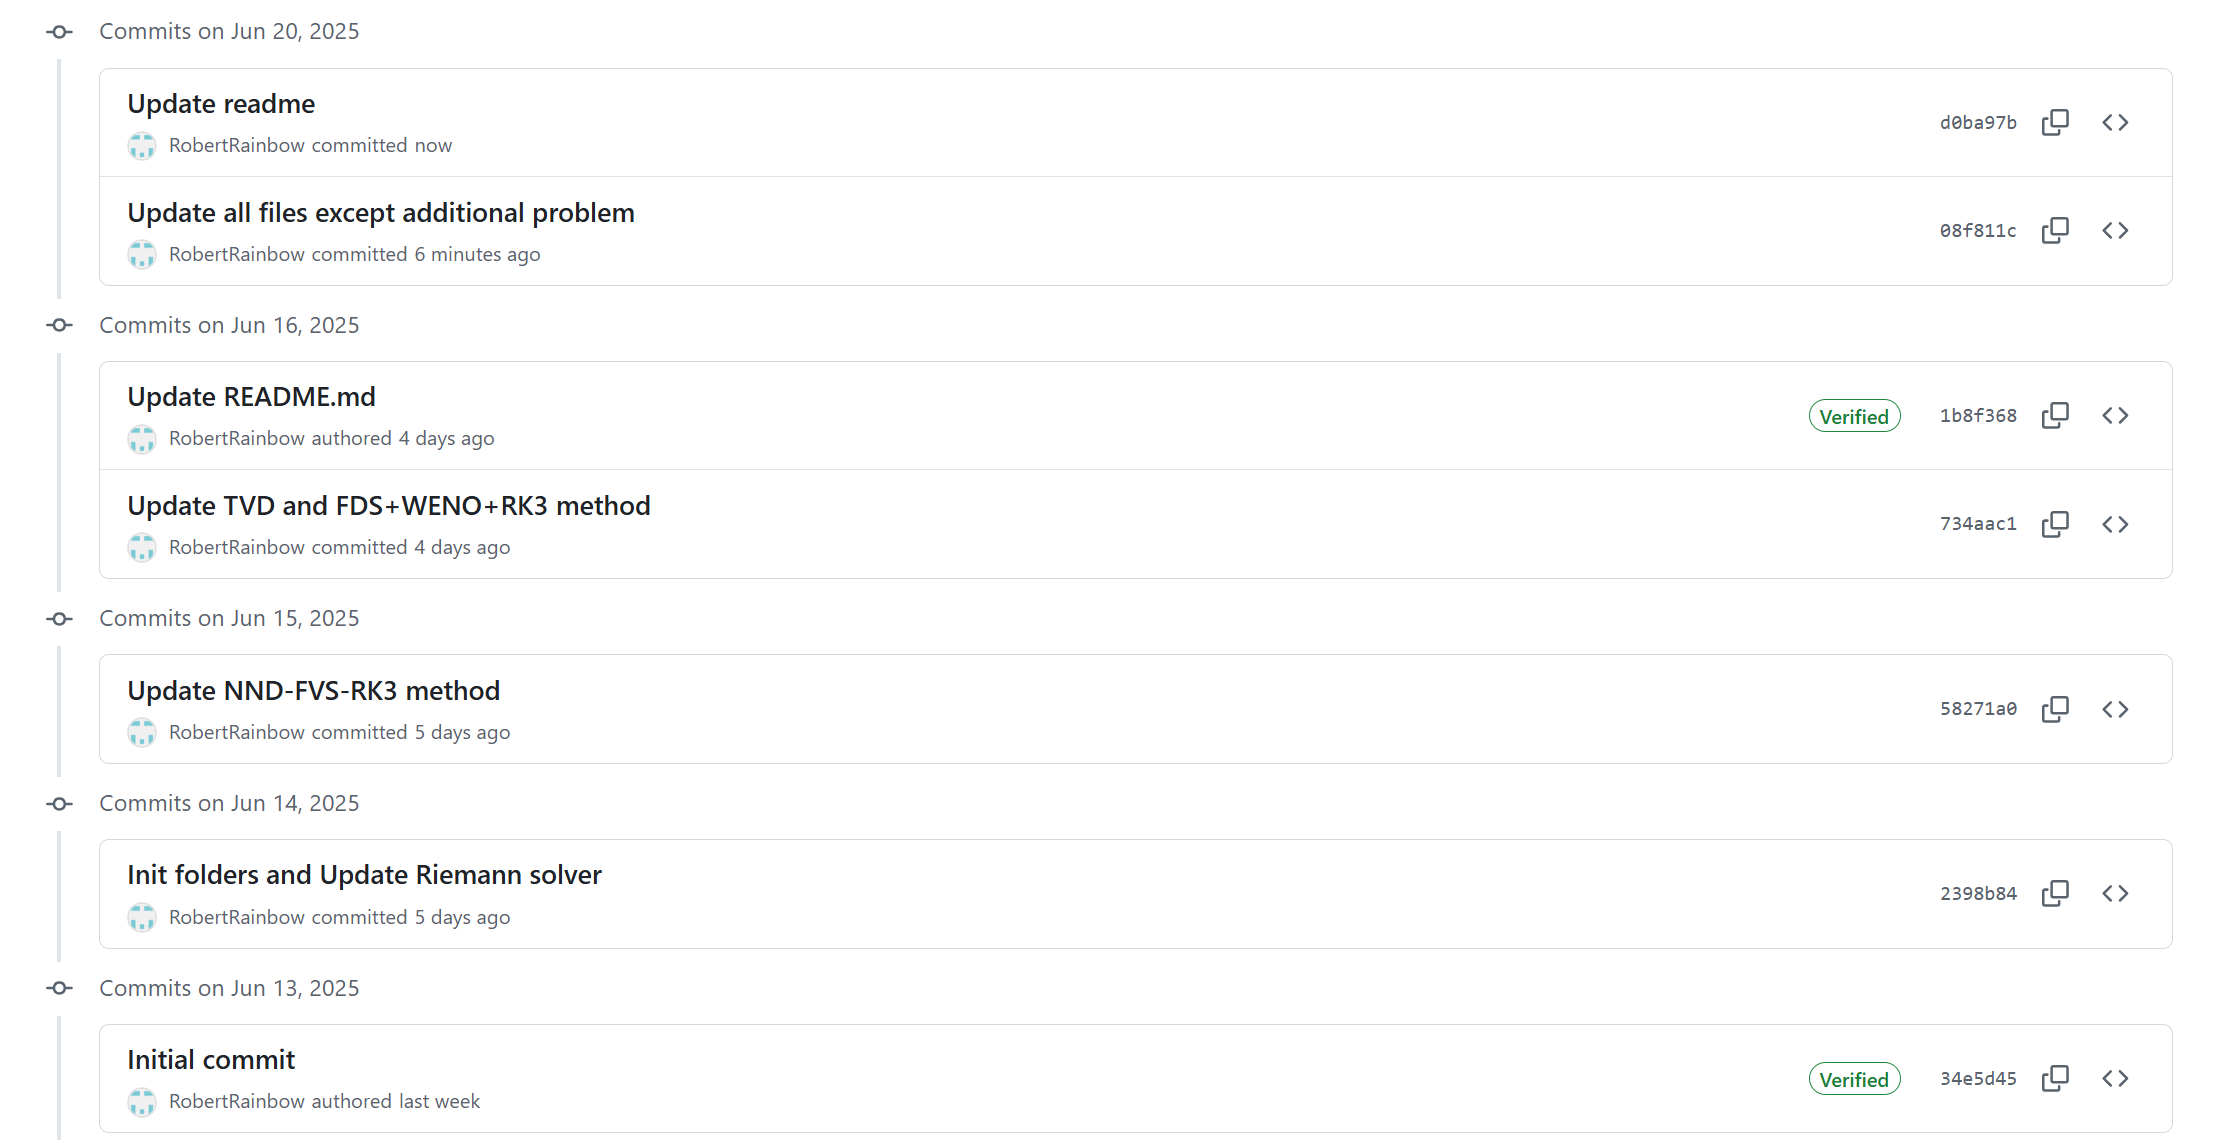
\includegraphics[width=\textwidth]{./fig/git.png}
					\caption{\fontsize{10pt}{15pt}\selectfont Github管理图}
				\end{minipage}
			\end{figure}
			
			\item AI使用说明:
			本项目在进行Riemann精确解分析的时候使用了AI+网络资料搜索的部分代码参考,在完成其余各部分matlab代码时均为自己查阅相关书籍与论文时推导并编写的。总AI代码量约占100/1000=10\%。具体AI工具使用表如下所示:
			\begin{table}[H]
				\centering
				\caption{AI工具使用声明表}
				\begin{tabular}{lcc}
					\toprule
					AI工具名称 & AI生成代码行数及功能 & 核心算法部分自主编写比例  \\
					\midrule
					ChatGPT       &  162行.功能:求解Riemann精确解 &    $1-\frac{162}{215+57+211+213+119+222+158=1195}=86.44\%$  \\
					\bottomrule
				\end{tabular}
			\end{table}
		\end{enumerate}
	
\end{document}

